The majority of this chapter will focus on the convection-diffusion problem using the abstract theory that we have discussed in the previous chapter. In particular, we shall use the DPG method based on the ultra-weak formulation with optimal test functions to solve this model problem and analyze its behavior as $\epsilon\rightarrow 0$. Our goal is to show the robustness of the method with respect to $\epsilon$, and demonstrate its usefulness as a numerical method for solving singular-perturbed problems. 

\section{DPG formulation for convection-diffusion}

\seclab{sec:modelSec}

The convection-diffusion problem is given on a domain
$\Omega \subset \mathbb{R}^d$ with boundary $\pO \equiv \Gamma$
\begin{equation}
\div (\beta u) - \epsilon\Delta u = f  \in \L \label{primal},
\end{equation}
which can be cast into the first order form on the group variable
$\LRp{u,\sigma}$ as
\begin{equation}
\eqnlab{CDstrong}
A \LRp{u,\sigma} \coloneqq \LRs {
\begin{array}{c}
\div (\beta u - \sigma) \\ \frac{1}{\epsilon}\sigma - \grad u
\end{array}} = \LRs{
\begin{array}{c}
f \\ 0
\end{array}
}.
\end{equation}
Using the abstract ultra-weak formulation developed in Section
\secref{abstractUweak} for the first order system of PDEs \eqnref{CDstrong} we
obtain
\begin{align*}
b\left(\left(u,\sigma, \widehat{u}, \widehat{f}_n\right),
\left( v, \tau \right)\right) = \left(u,\div \tau - \beta \cdot \grad
v\right)_{\Oh} + \left(\sigma, \epsilon^{-1} \tau + \grad v\right)_{\Oh} - \LRa{
\jump{\tau\cdot n}, \widehat{u} }_{\Gh} + \LRa{ \widehat{f}_n,
  \jump{v} }_{\Gh},
\end{align*}
where $\LRp{v, \tau}$ is the group test function. It should be pointed
out that the divergence and gradient operators are understood to act
element-wise on test functions $\LRp{v, \tau}$ in the broken graph
space $ D\LRp{A_h^*} \coloneqq  H^1(\Oh) \times H({\rm div}, \Oh)$, but
globally as usual on conforming test functions, i.e.\ $ \LRp{v, \tau}
\in  H^1(\Omega) \times H({\rm div}, \Omega)$. It follows that the
canonical test norm can be written as
\[
\|\left(v, \tau\right)\|_V^2 = \|\left(v, \tau\right)\|_{H^1(\Oh) \times H({\rm div},\Oh)}^2
= \sum_{K\in \Oh} \|\left(v, \tau\right)\|_{H^1(K) \times H({\rm
    div},K)}^2,
\]
where
\[
\|\left(v, \tau \right)\|_{H^1(K) \times H({\rm div},K)}^2 =
\|v\|_{L^2(K)}^2 + \|\grad v\|_{L^2(K)}^2 + \|\tau\|_{L^2(K)}^2 +
\|\div \tau\|_{L^2(K)}^2.
\]

In order to define the proper norm on the trial space, boundary
conditions need to be specified. We begin by splitting the boundary
$\Gamma$ as follows
\begin{align*}
\Gamma_{-} &\coloneqq \{x\in \Gamma; \beta_n(x) < 0\}, \quad {\rm
  (inflow)}\\ \Gamma_{+} &\coloneqq \{x\in \Gamma; \beta_n(x) > 0\},
\quad {\rm (outflow)}\\ \Gamma_{0} &\coloneqq \{x\in \Gamma;
\beta_n(x) = 0\},
\end{align*}
where $\beta_n \coloneqq \beta \cdot n$.
Previous work in \cite{DPGrobustness} adopted Dirichlet boundary
conditions everywhere on $\Gamma$.  
%and we could obtain the robustness only with special weighted norms in which the weight varied spatially. 
We employ instead the inflow
condition of Hesthaven \etal \cite{Hesthaven96astable}, where we set
\[
\beta_n u - \sigma_n  = u_0, \quad \text{on } \Gm,
\]
instead of $\beta_n u = u_0$. The former resembles the latter
as $\epsilon$ approaches zero\footnote{For our model problem, as for many problems of interest in computational fluid dynamics, we expect $\grad u$ to be small near the inflow, and that the solutions to \eqref{primal} using $\beta_n u - \sigma_n = f_n = u_0$ on $\Gamma_-$ will converge to that using $u=u_0$ on $\Gamma_-$  for sufficiently small $\epsilon$.}; however, the latter induces a more ``well-behaved" adjoint problem than the former, which, as we will discuss, affects the performance of DPG. 

On the outflow boundary, we apply standard homogeneous Dirichlet boundary conditions
\[
u = 0, \quad \text{on } \Gp.
\]
The material in this chapter is intended to act as an extension of the theory developed by Heuer and Demkowicz in \cite{DPGrobustness}. The primary focus of this chapter is to analyze the DPG method and extend previous results under this new choice of inflow boundary conditions. The difference in the performance of DPG under both new and old boundary conditions is connected to the difference in the adjoint problems induced under each boundary condition. The secondary contribution of this work will be to analyze the performance of DPG under a new mesh-dependent test norm. 

\subsection{Norms on $U$}

With the above boundary conditions at hand, the ultra-weak formulation
\eqnref{uweak} can be fitted in the abstract form \eqnref{variationEq}
as
\begin{align*}
b\left(\left(u,\sigma, \widehat{u}, \widehat{f}_n\right), \left( v,
\tau\right)\right) &= \left(u,\div \tau - \beta \cdot \grad
v\right)_{\Oh} + \left(\sigma, \epsilon^{-1} \tau + \grad
v\right)_{\Oh} \\
&- \LRa{ \jump{\tau\cdot n}, \widehat{u} }_{\Gh
  \setminus \Gp} + \LRa{ \widehat{f}_n, \jump{v} }_{\Gamma_h \setminus
  \Gm} =  \left(f, v\right) -
\LRa{ u_0, v }_{\Gamma_-} = l\left(\left(v, \tau\right)\right),
\end{align*}
which, after using the setting in Section \secref{abstractUweak},
suggests the following trial space (see \cite{analysisDPG, Bui-ThanhDemkowiczGhattas11b} for details):
\begin{align*}
u, \sigma \in \L, \quad \text{and } \LRp{\uh,\fnh} \in
\gamma\LRp{D\LRp{A}} \subset \gamma\LRp{  H^1(\Omega) \times
H({\rm div}, \Omega)} = H^{\frac{1}{2}}\left(\Gh\right) \times H^{-\frac{1}{2}}\left(\Gh\right).
\end{align*}
The space for $u$ and $\sigma$ are simply scalar and vector $L^2$ spaces over $\Omega$, while the space for $\left(\uh,\fnh\right)$ is the trace space of the graph space of the operator $A$ subject to the boundary conditions.

The minimum energy extension norm \eqnref{MEnorm} now reads
\begin{align*}
\|\widehat{u}\| &= \inf_{w\in H^1(\Omega),
  \left.w\right|_{\Gamma_+}=0, \left.w\right |_{\Gh\setminus
    \Gamma_+ } = \widehat{u}} \|w\|_{H^1(\Omega)}, \\ \|\widehat{f}_n\|
&= \inf_{q\in H({\rm div},\Omega), \left.q\cdot n\right|_{\Gamma_-}=
  0, \left. q\cdot n \right |_{\Gh\setminus
    \Gamma_-} = \widehat{f}_n}
\|q\|_{H({\rm div},\Omega)}.
\end{align*}
As a result, the canonical norm on $U$ is given by
\[
\left\|\left(u,\sigma,\widehat{u},\widehat{f}_n\right)\right\|_U^2 = 
\|u\|_{L^2(\Oh)}^2 + \|\sigma\|_{L^2(\Oh)}^2 +
\|\widehat{u}\|^2 + \|\widehat{f}_n\|^2.
\]

\subsection{Norms on $V$}

%We will denote $\|\cdot \| = \|\cdot\|_{L^2}$ for all functions defined on $\Oh$. 
As $\tau \in H({\rm div},\Oh)$ and $v \in H^1(\Oh)$, we will
construct norms on $v$ and $\tau$ 
which are equivalent to the canonical $H^1(K) \times H({\rm div},K)$
norm over a single element
\[
\|\left(v,\tau\right)\|_{H^1(K) \times H({\rm div},K)}^2 =
\|v\|_{L^2(K)}^2 + \|\grad v\|_{L^2(K)}^2 + \|\tau\|_{L^2(K)}^2 +
\|\div \tau\|_{L^2(K)}^2.
\]
The squared norm over the entire triangulation $\Oh$ is defined to be the squared sum of contributions from each element
\[
\|\left(v,\tau\right)\|_{H^1(\Oh) \times H({\rm div},\Oh)}^2
= \sum_{K\in \Oh} \|\left(v,\tau\right)\|_{H^1(K) \times H({\rm
    div},K)}^2.
\]
The exact norms that we will specify on $V$ will be determined later. 

The norms on the skeleton $\Gh$ for $v$ and $\tau$ are defined by duality from the bilinear form
\begin{align*}
\left\|\jump{\tau\cdot n}\right\| &= \left\|\jump{\tau\cdot n}\right\|_{\Gh \setminus \Gamma_+} \coloneqq \sup_{w\in H^1(\Omega), \left.w\right|_{\Gamma_+} = 0} \frac{\langle \jump{\tau \cdot n}, w\rangle}{\|w\|_{H^1(\Omega)}},\\
\left\|\jump{v}\right\|&=\left\|\jump{v}\right\|_{\Gh^0 \cup \Gamma_+} \coloneqq \sup_{\eta\in H({\rm div},\Omega), \left.\eta\cdot n\right|_{\Gamma_- \cup \Gamma_0} = 0} \frac{\langle \jump{v}, \eta\cdot n\rangle}{\|\eta\|_{H({\rm div},\Omega)}}.
\end{align*}

\subsection{Approximability of the quasi-optimal test norm}
%\textcolor{blue}{need to define what we mean by robustness. perharps the best place is in the introduction}
An obvious choice for the test norm would be the quasi-optimal norm; it is the canonical test norm, and DPG has been shown to be well-posed and robust under such an optimal test norm for a large class of problems \cite{DPGrobustness,Bui-ThanhDemkowiczGhattas11b, stokesDPG}. However, computations with the quasi-optimal test norm for convection-diffusion problems turn out to be quite problematic for small diffusion and coarse meshes.  

For convection-diffusion, the quasi-optimal test norm is 
\[
\|\left(v,\tau\right)\|_V^2 = \| \div \tau - \beta \cdot \grad v
\|_{L^2}^2 + \| \epsilon^{-1} \tau + \grad v \|_{L^2}^2 +
\|v\|_{L^2}^2 + \|\tau\|_{L^2}^2.
\]
%We note that the optimal test norm will automatically guarantee the
%robust bound $\|\left(\tau, v\right)\|_V \leq \|u\|_{L^2}$.
Use of this norm for the convection-diffusion problem is difficult --- since the problem \eqnref{optvVar} for optimal test functions is local, we can transform the problem over a single element $K$ to the reference element $\widehat{K}$ and show that it is equivalent to a reaction-diffusion system, with diffusion parameter $\frac{\epsilon}{|K|}$, where $|K|$ is the element measure \cite{DBLP:journals/procedia/NiemiCC11}. We refer to the inverse of this parameter $\frac{|K|}{\epsilon}$ as the element Peclet number $\rm Pe$. For a coarse mesh and small diffusion parameter $\epsilon$, we will have a large element Peclet number, and optimal test functions under the quasi-optimal test norm will develop strong boundary layers of width $\rm Pe$, as seen in Figure~\ref{fig:optTestBoundary}.

In the application of DPG in \cite{DPG1,DPG2,DPG3,DPG4}, the approximation of optimal test functions is done using polynomial enrichment. We search for the solution to \eqnref{optvVar} in the enriched test space $\tilde{V} \approx \prod_{K} P^{p+\Delta p}(K)$, where $p$ is the polynomial order of the trial space on a given element $K$.\footnote{$V$ is only \emph{approximately} equal to the space $\prod_{K} P^{p+\Delta p}(K)$. In practice, $V$ is constructed using locally $H^1$-conforming and Raviart-Thomas elements of appropriate order.}  In other words, optimal test functions are approximated element-by-element using polynomials whose order is $\Delta p$ more than the local order of approximation.  Under this scheme, the error in approximation of test functions is tied to the effectiveness of the $p$-method.  Unfortunately, for problems with boundary layers --- including the approximation of test functions under the quasi-optimal test norm --- the $p$-method performs very poorly. As a result of this poor approximation, the numerical solutions of the convection-dominated diffusion equation under DPG using the quasi-optimal test norm tend to be of poor quality, and do not exhibit all the proven properties of DPG (for example, the energy error may increase after mesh refinement, even though, by virtue of DPG delivering a best approximation, the energy error for a coarse mesh must be greater than or equal to the energy error for a finer mesh).  We conclude that the error in approximation of optimal test functions using simple polynomial enrichment pollutes and ruins the performance of DPG under the quasi-optimal test norm. 

\begin{figure}[!h]
\centering
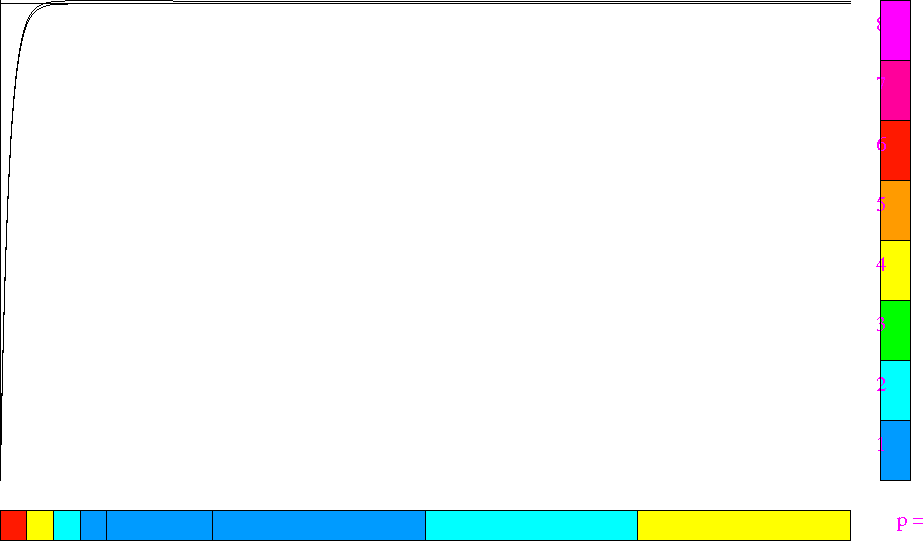
\includegraphics[scale=.25]{figs/opt.png}
\caption{$v$ and $\tau$ components of the 1D optimal test functions corresponding to the flux $\widehat{f}_n$ on the right-hand side of a unit element for $\epsilon = 0.01$. The solution has been obtained using automatic $hp$-adaptivity driven by the test norm with the error tolerance set at 1\%.}
\label{fig:optTestBoundary}
\end{figure}

The difficulty in using the quasi-optimal test norm for convection-diffusion is perplexing at first, considering that the quasi-optimal norm has yielded excellent results for the Helmholtz equation and other wave propagation problems.  The difference between the two problems lies in the fact that, for wave propagation problems, the mesh size tends to be on the order of the wavenumber $k$ --- the singular perturbation parameter. Transforming the variational problem using the quasi-optimal test norm for wave propagation yields smooth optimal test functions that are approximated much more accurately using only polynomials over the reference element. Typically, the wavenumbers $k$ of physical interest are $O(100)$ with respect to a unit domain. The corresponding finite element problems will typically be solved on meshes containing approximately $O\!\left(k^d\right)$ elements in $\mathbb{R}^d$, well within the range of a computationally tractable simulation. However, for convection diffusion problems, the relevant range of $\epsilon$ for physical problems can be as small as $1e-7$. Solving on under-resolved meshes is thus unavoidable, and the approximability of optimal test functions must be addressed in order to take advantage of the properties of DPG.

Resolving such boundary layers present in test functions under the quasi-optimal test norm has been investigated numerically using specially designed (Shishkin) subgrid meshes by Niemi, Collier, and Calo in
\cite{DBLP:journals/procedia/NiemiCC11}.  However, even with Shishkin meshes, the approximation of optimal test functions under the quasi-optimal norm is far more expensive and complex to implement than approximation of test functions using a simple $p$-enriched space for $V$. We therefore aim instead to design a test norm that does not induce boundary layers, but still delivers good approximation results over a range of $\epsilon$.  

\subsection{Analysis of a DPG test norm}
\seclab{sec:testNormSec}
We are interested in computing DPG optimal test functions for the convection-diffusion equation with very small values of $\epsilon$; due to the difficulty of approximating optimal test functions, we conclude that the use of the quasi-optimal test norm is infeasible towards this goal. 

However, if we naively choose a test norm that does not generate boundary layers, the performance of DPG may be adversely affected. For example, if $\|\left(v,\tau\right)\|_V^2 = \|v\|_{H^1(\Omega_h)}^2 + \|\tau\|^2_{H({\rm div},\Omega_h)}$, the $H^1(\Omega_h)\times H({\rm div},\Omega_h)$ norm, then the corresponding test functions will be smooth and free of boundary layers; however, the performance of DPG will provide approximations which worsen in quality as $\epsilon$ becomes very small \cite{DPG3,DPGrobustness}. 

Our goal is to construct a test norm that compromises between performance of DPG and approximability of test functions.  This test norm should not produce boundary layers in the optimal test functions, but still induce an energy norm that yields good approximation properties for small $\epsilon$. We note that, even under the quasi-optimal norm, the norms on the flux and trace variables will likely depend on $\epsilon$. Thus, we aim to construct a test norm for which the DPG method will be robust in $\epsilon$ with respect to the \emph{field variables}. 

For now, we discuss the steps necessary to analyze the performance of DPG with respect to a non-canonical test norm. We require a priori that the test norm has separable $\tau$ and $v$ components --- in other words, that there are no terms in the test norm that couple $\tau$ and $v$ together. Problem \eqnref{optvVar} then decouples, such that the components of the vector-valued test function $\left(v,\tau\right)$ can be solved for independently of each other. The decoupled variational problems are no longer systems but scalar equations in $\tau$ and $v$, for which it is easier to conclude whether or not there are boundary layers in the solutions (the avoidance of boundary layers in the test norm will be discussed in more detail in Section~\ref{sec:num_exp}, which describes our numerical experiments). \textbf{This will ensure that the resulting DPG method does not suffer from approximation errors in the optimal test functions}.

We begin with the following test norm:
\[
\left\|\left(v,\tau\right)\right\|^2_V \coloneqq \|v\|_{L^2}^2 + \epsilon\|\grad v\|_{L^2}^2 + \|\beta \cdot \grad v\|_{L^2}^2  + \frac{1}{\epsilon}\|\tau\|_{L^2}^2 + \|\div \tau\|_{L^2}^2.
\]
The use of this norm is problematic for practical computations; we will discuss the reasons why and present a modification of it in Section~\secref{sec:meshDep}. 

We can see how this norm will differ from the canonical $H^1(\Omega_h)\times H({\rm div},\Omega_h)$ norm: the clearest difference is the fact that the gradient in the streamline direction is $O(1)$, while the full gradient is $O(\sqrt{\epsilon})$, so that, in our test norm, the streamline gradient of $v$ will be emphasized over the full gradient of $v$ for small $\epsilon$. 

The choice of this test norm is implied by the mathematics of the adjoint problem. Roughly speaking, necessary conditions for the performance of DPG to not degenerate as $\epsilon \rightarrow 0$ are derived through analysis of specific test functions. For example, if $u$ is the first $L^2$ component of the solution to the variational problem defined in Section~\secref{sec:modelSec}, by choosing $(v,\tau) \in H^1(\Omega) \times H({\rm div},\Omega)$ such that 
\begin{align*}
\div \tau - \beta \cdot \grad v &= u \\
\frac{1}{\epsilon} \tau - \grad v &= 0,
\end{align*}
we have
\[
 \nor{u}_{L^2}^2 = b\left(\left(u,\sigma,\widehat{u},\widehat{f}_n\right),\left(v,\tau\right)\right) \leq \nor{\left(u,\sigma,\widehat{u},\widehat{f}_n\right)}_{U,V} \nor{\left(v,\tau\right)}_V,
\]
and we recover the $L^2$ norm of $u$ from the bilinear form.

Let $\|a\| \lesssim \|b\|$ denote an $\epsilon$-independent bound; specifically, that $\|a\| \leq C\|b\|$ for a constant $C$ independent of $\epsilon$. Consequently, if for any $u\in L^2(\Oh)$, $\nor{\left(v,\tau\right)}_V\lesssim \nor{u}_{L^2}$, then dividing through by $\nor{u}_{L^2}$ gives the bound
\[
 \nor{u}_{L^2} \lesssim \nor{\left(u,\sigma,\widehat{u},\widehat{f}_n\right)}_E.
\]
In other words, there is the guarantee that the $L^2$ error in $u$ is at least robustly bounded from above by the energy error. Then, if the energy error (which DPG minimizes) approaches zero, the $L^2$ error in $u$ will as well. The same exercise can be repeated for the stress $\sigma$, as well as the flux variables $\widehat{u}$, $\widehat{f}_n$. 

This methodology gives constraints on the quantities found in the test norm; any quantity present in $\nor{\left(v,\tau\right)}_V$ must be shown to be bounded from above independently of $\epsilon$ by the load of the adjoint problem. However, showing this simply amounts to showing \textit{standard energy estimates} for $H^1$ and $H({\rm div})$-conforming finite elements. A more detailed discussion on the reasoning behind the construction of test norms can be found in \cite{DPGrobustness}. 

The second step will be to \textbf{show the equivalence of the energy norm to explicit norms on $U$}. Since we do not generally have a closed form expression for the DPG energy norm, we seek to understand the behavior of DPG by finding a norm on $U$ to which the DPG energy norm is equivalent. Since $\left(u,\sigma,\widehat{u},\widehat{f}_n\right)\in U$ is a group variable from a tensor product space, we construct norms on $U$ through the combination of norms on $u$, $\sigma$, $\widehat{u}$, and $\widehat{f}_n$. Specifically, we use the norm on $U$ 
\begin{equation}
\left\| \left(u,\sigma,\widehat{u},\widehat{f}_n\right)\right \|_{U}^2 \coloneqq \|u\|^2 + \|\sigma\|^2 + \left\|\widehat{u}\right\|^2 + \left\|\widehat{f}_n\right\|^2.
\end{equation}
For equivalence between norms, two constants are specified. However, since this norm on $U$ is a norm on four separate variables, we can specify not just two but eight equivalence constants.\footnote{Sharper estimates are attainable if these constants are allowed to vary over the mesh $\Oh$. See Section~\ref{sec:main_bounds} for a discussion.} In order to simplify analysis, we phrase this equivalence statement in an alternative form. 

Let $\nor{\cdot}_E \coloneqq \nor{\cdot}_{U,V}$, the energy norm induced by the test norm described above. We seek the bound of $\nor{\cdot}_E$ from above and below:
\[
\left\| \left(u,\sigma,\widehat{u},\widehat{f}_n\right)\right \|_{U,1} \lesssim  \left\| \left(u,\sigma,\widehat{u},\widehat{f}_n\right)\right \|_E \lesssim \left\| \left(u,\sigma,\widehat{u},\widehat{f}_n\right)\right \|_{U,2},
\]
where both $\|\cdot\|_{U,1}$ and $\|\cdot\|_{U,2}$ are defined as scaled combinations of the norms on $u, \sigma, \widehat{u}$, and $\widehat{f}_n$
\begin{equation}
\eqnlab{uNorms}
\left\| \left(u,\sigma,\widehat{u},\widehat{f}_n\right)\right \|_{U,i}^2 \coloneqq \left(C_u^i\|u\|\right)^2 + \left(C_\sigma^i\|\sigma\|\right)^2 + \left(C_{\widehat{u}}^i\|\widehat{u}\|\right)^2 + \left(C_{\widehat{f}_n}^i\|\widehat{f}_n\|\right)^2,\quad i = 1,2
\end{equation}
Our goal is to explicitly derive the equivalence constants 
%$C^1_u,\ldots, C^1_{\widehat{f}_n}$ and $C^2_u,\ldots, C^2_{\widehat{f}_n}$ 
that define the norms $\|\cdot\|_{U,1}$ and $\|\cdot\|_{U,2}$ respectively, taking into account any dependency on $\epsilon$. To do so, we need a relation between trial norms on $U$ and test norms on $V$.

Recall from Section~\secref{energyPair} that every test norm induces a corresponding trial norm, and vice versa. Let $\|\cdot\|_{U,1} \simeq \|\cdot\|_{U,2}$ mean that the norms $\|\cdot\|_{U,1}$ and $\|\cdot\|_{U,2}$ are equivalent, with equivalence constants independent of $\epsilon$. By equivalence of finite dimensional norms and the discussion in Section~\secref{energyPair} on the duality between test norms/energy norms, the norms \eqnref{uNorms} on $U$ induce the equivalent test norms on $\left(v,\tau\right) \in H^1(\Oh)\times H({\rm div},\Oh)$
\begin{align*}
\left\|\left(v,\tau\right)\right\|_{V,{U,i}} &\simeq \sup_{\left(u,\sigma,\widehat{u},\widehat{f}_n\right)\in U}\frac{b\left(\left(u,\sigma,\widehat{u},\widehat{f}_n\right),\left(v,\tau\right)\right)}{C_u^i\|u\| + C_\sigma^i\|\sigma\| + C_{\widehat{u}}^i\|\widehat{u}\|+ C_{\widehat{f}_n}^i\|\widehat{f}_n\|}\\
&= \sup_{\left(u,\sigma,\widehat{u},\widehat{f}_n\right)\in U}\frac{\left(u,\div \tau - \beta \cdot \grad v\right) + \left(\sigma, \epsilon^{-1} \tau + \grad v\right) - \langle \jump{\tau_n}, \widehat{u} \rangle_{\Gamma_-\cup \Gh^0} + \langle \widehat{f}_n, \jump{v} \rangle_{\Gamma_+ \cup \Gh^0}}{C_u^i\|u\| + C_\sigma^i\|\sigma\| + C_{\widehat{u}}^i\|\widehat{u}\|+ C_{\widehat{f}_n}^i\|\widehat{f}_n\|}\\
& \simeq \frac{1}{C_u^i}\|g\| + \frac{1}{C_\sigma^i}\|f\| + \frac{1}{C_{\widehat{u}}^i}\sup_{\widehat{u}\neq 0, \left.\widehat{u}\right|_{\Gamma_+} = 0} \frac{\langle \jump{\tau\cdot n}, \widehat{u}\rangle}{\|\widehat{u}\|} +\frac{1}{C_{\widehat{f}_n}^i}\sup_{\widehat{f}_n\neq 0, \left.\widehat{f}_n\right|_{\Gamma_-}=0}\frac{\langle \widehat{f}_n, \jump{v}\rangle}{\|\widehat{f}_n\|},
\end{align*}
where $f$ and $g$ are defined element-wise over $\Oh$ as 
\begin{align*}
g &\coloneqq \div \tau - \beta \cdot \grad v\\
f &\coloneqq \epsilon^{-1}\tau + \grad v.
\end{align*}
By definition of the norms on the quantities defined on the skeleton $\Gh$, this gives the characterization of the induced test norm 
\[
\|\left(v,\tau\right)\|_{V,{U,i}} \simeq \frac{1}{C_u^i}\|g\| + \frac{1}{C_\sigma^i}\|f\| + \frac{1}{C_{\widehat{u}}^i}\|\jump{\tau\cdot n}\| + \frac{1}{C_{\widehat{f}_n}^i}\|\jump{v}\|, \quad i = 1,2.
\]
We can now use this relation to compare different norms on $U$ by comparing their induced norms on $V$ (recall that showing a robust inequality between two norms on $U$ is equivalent to showing the robust \textit{reverse} inequality in the induced norms on $V$). Namely, we can show the bound of $\nor{\cdot}_{U,1} \lesssim \nor{\cdot}_E$ by showing the bound $\nor{\left(v,\tau\right)}_{V,U,1} \gtrsim \nor{\left(v,\tau\right)}_{V}$, and likewise for $\nor{\cdot}_E \lesssim \nor{\cdot}_{U,2}$. 

Since the techniques used to show such bounds are more involved, we break the procedure up into two steps:
\begin{enumerate}
\item{}Decompose test functions $(v,\tau)$ into three separate, more easily analyzable components (Section~\ref{sec:strategy2}).
\item{}Derive adjoint estimates (Section~\ref{sec:strategy3}).
\end{enumerate}

\subsubsection{Decomposition into analyzable components}
\label{sec:strategy2}

Having reduced the problem of comparing norms on $U$ to the comparison of norms on $V$, we break the analysis of $\left(v,\tau\right) \in V$ into the analysis of three subproblems.  Define the decomposition
\[
\left(v,\tau\right) = \left(v_0,\tau_0\right) + \left(v_1,\tau_1\right) + \left(v_2,\tau_2\right),
\]
where $\left(v_1,\tau_1\right)$ satisfies 
\begin{align*}
\epsilon^{-1}\tau_1 + \grad v_1 &= 0 ,\\
\div \tau_1 - \beta\cdot \grad v_1 &=  \div \tau - \beta\cdot \grad v = g, 
\end{align*} 
and $\left(v_2,\tau_2\right)$ satisfies
\begin{align*}
\epsilon^{-1}\tau_2 + \grad v_2 &= \epsilon^{-1}\tau + \grad v = f, \\
\div \tau_2 - \beta\cdot \grad v_2 &= 0.
\end{align*}
Both $(v_1,\tau_1), (v_2,\tau_2) \in H({\rm div}; \Omega)\times H^1(\Omega)$ are understood to satisfy these relations in a conforming sense over the domain $\Omega$; however, the divergence of $\tau$ and gradient of $v$ on the right hand side are still understood to be taken in an element-wise fashion. 

We will additionally require both $\left(v_1,\tau_1\right), \left(v_2,\tau_2\right)$ to satisfy the adjoint homogeneous boundary conditions
\begin{align}
\tau_i\cdot n &= 0, \quad \text{on }\Gamma_- \label{bc_1}\\
v_i &= 0, \quad \text{on } \Gamma_+ \label{bc_2}
\end{align}
for $i = 1, 2$. The selection of $H({\rm div}, \Omega)\times H^1(\Omega)$ conforming test functions satisfying the specific boundary conditions above removes the contribution of the jump terms over the skeleton $\Gh$ in the bilinear form, allowing us to analyze field terms in the induced test norms separately from  the boundary/jump terms. 

Finally, by construction, $\left(v_0,\tau_0\right) \in H^1(\Oh) \times H({\rm div},\Oh)$ must satisfy 
\begin{align*}
\epsilon^{-1}\tau_0 + \grad v_0 &= 0\\
\div \tau_0 - \beta\cdot \grad v_0 &= 0
\end{align*}
with jumps
\begin{align*}
\jump{v_0} &= \jump{v}, \quad \text{on }\Gh^0\\
\jump{\tau_0 \cdot n} &= \jump{\tau \cdot n}, \quad \text{on }\Gh^0.
\end{align*}
and boundary conditions
\begin{align*}
v_0 &= v, \quad \text{on } \Gamma_+ \\
\tau_0 \cdot n &= \tau \cdot n, \quad \text{on } \Gamma_-\cup \Gamma_0. 
\end{align*}
Notice that the evaluation the bilinear form $b\left(\left(u,\sigma,\widehat{u},\widehat{f}_n\right),\left(v,\tau\right)\right)$ with each specific test functions returns only one part of the bilinear form. Furthermore, by choosing the proper loads $g = u$ and $f=\sigma$, we can recover from the bilinear form the norms of $u$ and $\sigma$ (as described in Section~\secref{sec:testNormSec}), as well as the norms on $\widehat{u}$, and $\widehat{f}_n$.\footnote{To recover the norms on $\widehat{u}$, and $\widehat{f}_n$, the loads $f$, and $g$ must be zero, and the jumps of the test function $(v,\tau)$ must be chosen specifically.}

We have now decomposed an arbitrary test function $\left(\tau,v\right)$ into a discontinuous contribution and two continuous contributions.  Recall that our goal is to show the robust bound from above and below of the DPG energy norm by $\|\cdot \|_{U,1}$ and $\|\cdot \|_{U,2}$:
\[
\left\| \left(u,\sigma,\widehat{u},\widehat{f}_n\right)\right \|_{U,1} \lesssim  \left\| \left(u,\sigma,\widehat{u},\widehat{f}_n\right)\right \|_E \lesssim \left\| \left(u,\sigma,\widehat{u},\widehat{f}_n\right)\right \|_{U,2}.
\]

Under the duality of trial and test norms and the decomposition of test functions $\left(\tau,v\right) \in V$ into $\left(\tau_0,v_0\right), \left(\tau_1,v_1\right)$, and $\left(\tau_2,v_2\right)$, the above bound is equivalent to bounding each component 
\begin{align*}
\|\left(v,\tau\right)\|_{V,U,1} &\gtrsim \sum_{i=0}^2\|\left(v_{i},\tau_{i}\right)\|_V \gtrsim \|\left(v,\tau\right)\|_{V,U,2}.
%\|\left(v,\tau\right)\|_{V,1} &\lesssim \|\left(v_{1},\tau_{1}\right)\|_V \lesssim \|\left(v,\tau\right)\|_{V,2}\\
%\|\left(v,\tau\right)\|_{V,1} &\lesssim \|\left(v_{2},\tau_{2}\right)\|_V \lesssim \|\left(v,\tau\right)\|_{V,2}
\end{align*}
Bounding $\|\left(v_0,\tau_0\right)\|$ requires the use of techniques first developed in \cite{analysisDPG} and adapted to convection-diffusion in \cite{analysisDPG} and \cite{DPGrobustness}. However, since $\left(\tau,v\right) \in H({\rm div}, \Omega)\times H^1(\Omega)$, the bound from above of test functions $\|\left(v_{1},\tau_{1}\right)\|_V$ and $\|\left(v_{2},\tau_{2}\right)\|_V$ is reduced to proving classical error estimates for the adjoint equations
\begin{align*}
\epsilon^{-1}\tau_1 + \grad {v_1} &= 0 \\
\div {\tau_1} - \beta\cdot \grad {v_1} &=  g, \\
\left.\tau_1\cdot n\right|_{\Gamma_-} &= 0, \\
\left.v_1\right|_{\Gamma_+} &= 0.
\end{align*} 
and 
\begin{align*}
\epsilon^{-1}\tau_2 + \grad {v_2} &= f \\
\div {\tau_2} - \beta\cdot \grad {v_2} &= 0, \\
\left.\tau_2\cdot n\right|_{\Gamma_-} &= 0, \\
\left.v_2\right|_{\Gamma_+} &= 0.
\end{align*} 
More generally, we can analyze the adjoint equations
\begin{align}
\epsilon^{-1}\tau + \grad {v} &= f \label{adjoint1}\\
\div {\tau} - \beta\cdot \grad {v} &= g, \label{adjoint2}
\end{align}
for arbitrary data $f, g\in L^2({\Omega})$ and boundary conditions $\jump{\tau\cdot n}_{\Gamma_-} = 0$ and $\jump{v}_{\Gamma_+} = 0$.  In other words, we want to analyze the stability properties of the adjoint equations by deriving bounds of the form $\|\left(v_1,\tau_1\right)\|_V\lesssim \|g\|_{L^2}$ and $\|\left(v_2,\tau_2\right)\|_V \lesssim \|f\|_{L^2}$.  

%An alternate interpretation of the above decomposition is that each component $(v_i,\tau_i)$ of the decomposition corresponds to a term in the bilinear form. For example, . If we evaluating our bilinear form with $(v,\tau) = (v_1,\tau_1)$ delivers
%\[
%b\left(\left(u,\sigma, \widehat{u}, \widehat{f}_n\right),
%\left( v_1, \tau_1 \right)\right) = (u,g)_{L^2} 
%\]
%By choosing $g = u$, 

\subsubsection{Adjoint estimates}
\label{sec:strategy3}

The final step to estimating the induced norm on $U$ by a selected localizable test norm on $V$ is to derive adjoint stability estimates on $\tau$ and $v$ in terms of localizable normed quantities.  We will construct complete test norms on $V$ through combinations of these normed quantities.%, where each normed quantity on $\tau$ or $v$ will correspond roughly to $\|u\|_{L^2}$, $\|\sigma\|_{L^2}$, $\|\widehat{u}\|$, or $\|\widehat{f}_n\|$.  

We introduce first the bounds derived; the proofs will be given later. For this analysis, it will be necessary to assume certain technical conditions on $\beta$.  For each proof, we require $\beta \in C^2(\bar{\Omega})$ and $\beta, \div \beta = O(1)$.  Additionally, we will assume that some or all of the following assumptions hold:
\begin{align}
&\curl \beta = 0, \quad 0<C \leq \left | \beta\right |^2 + \frac{1}{2}\div \beta, \quad C = O(1) \label{a_req},\\
&\grad \beta + \grad \beta ^T - \div \beta I = O(1) \label{b_req},\\
&\div \beta = 0 \label{c_req}.
\end{align}
Under proper assumptions on $\beta$, we have the robust bounds, which are proved in the Appendix. 
\begin{itemize}
\item \textbf{Lemma \ref{lemma_stream}}: \textit{For $\beta$ satisfying \eqref{a_req} and \eqref{b_req}, %$f=0$ 
and $v_1 \in H^1(\Omega)$, satisfying equations \eqref{adjoint1} and \eqref{adjoint2} with $f=0$, and with boundary conditions \eqref{bc_1} and \eqref{bc_2}},
\begin{align*}
\|\beta \cdot \grad v_1 \| &\lesssim \| g\|.
\end{align*}
Similarly, from $\div \tau_1 - \beta\cdot \grad v_1 = g$, we get $\|\div \tau_1\| \lesssim \|g\|$ as well.  
\item \textbf{Lemma \ref{lemma_grad}}: \textit{For $\beta$ satisfying \eqref{a_req}, and $v \in H^1(\Omega)$ satisfying equations \eqref{adjoint1} and \eqref{adjoint2} and boundary conditions \eqref{bc_1} and \eqref{bc_2}, and for sufficiently small $\epsilon$},
\[
\epsilon \|\grad v\|^2 + \|v\|^2 \lesssim \|g\|^2 + \epsilon \|f\|^2.
\]
We can characterize both $v_1$ and $v_2$ in the above decompositions using this theorem by setting either $f=0$ or $g=0$. 
%\begin{align*}
%\epsilon \|\grad v_1\|^2 + \|v_1\|^2 &\lesssim \|g\|^2\\
%\epsilon \|\grad v_2\|^2 + \|v_2\|^2 &\lesssim \epsilon \| f\|^2.
%\end{align*}
%By the triangle inequality, this implies for any $w$ of the form $w=v_1+v_2$
%\begin{align*}
%\epsilon \|\grad w\|^2 + \|w\|^2 &\lesssim \|g\|^2 + \epsilon \| f\|^2
%\end{align*}
\item \textbf{Lemma \ref{lemma_boundary}}: \textit{For $\beta$ satisfying \eqref{a_req}, \eqref{c_req}, and solutions $v_0 \in H^1(\Oh)$ and $\tau_0 \in H({\rm div},\Oh)$ of equations \eqref{adjoint1} and \eqref{adjoint2} with $f=g=0$,} 
\begin{align*}
\|\grad v_0\| = \frac{1}{\epsilon}\|\tau_0\| &\lesssim \frac{1}{\epsilon} \| \jump{\tau_0\cdot n}\|_{\Gh \setminus \Gamma_+} + \frac{1}{\sqrt{\epsilon}} \| \jump{v_0}\|_{\Gh^0 \cup \Gamma_+}.
\end{align*}
\end{itemize}
We are interested in showing the equivalence of the DPG energy norm with norms $\|\cdot\|_{U,1}$ and $\|\cdot\|_{U,2}$, respectively.  We will show this by bounding $\|\cdot \|_V$ from below by $\|\cdot\|_{V,U,1}$ and from above by $\|\cdot\|_{V,U,2}$ (the induced test norms for $\|\cdot\|_{U,1}$ and $\|\cdot\|_{U,2}$, respectively).  

%We will use Lemmas \ref{lemma_stream}, \ref{lemma_grad}, and \ref{lemma_boundary} to prove such bounds on our yet-unspecified test norm $\|(\tau,v)\|_V$. 

%Together, these estimates will be sufficient to construct a complete norm on $V$ and demonstrate bounds on induced test norms for different scalings of norms on $U$.  
%\tanbui{}{again, using the same notation
%  $(v, \tau)$ for all three problems is not a good idea. Why don't we
%  use $(v_i,\tau_i)$ introduced above? Things are much clearer this
%  way?}
\subsubsection{A mesh-dependent test norm}
\seclab{sec:meshDep}
Ideally, we would be interested in the use of the test norm 
\[
\|\left(v,\tau\right)\|_{V}^2 = \|v\|^2 + \epsilon \|\grad v\|^2 + \|\beta \cdot \grad v\|^2 + \| \div \tau\|^2 + \frac{1}{\epsilon}\|\tau\|^2
\]
for practical computations. However, the presence of the term $\|v\|$ together with $\sqrt{\epsilon}\|\grad v\|$ (and similarly $\|\div \tau\|$ and $\frac{1}{\sqrt{\epsilon}}\|\tau\|$ terms) induces boundary layers in the optimal test functions for under-resolved meshes. We can see this by recovering the strong form of the variational problem defining test functions. We first note that the variational problems for the $v$ and $\tau$ components of optimal test functions decouple from each other under this test norm. Then, examining the variational problem for the $v$ component only of an optimal test function, and assuming $\div \beta = 0$ for illustrative purposes, we have 
\begin{align*}
\left(\left(v,0\right),\left(\delta v,\delta\tau\right)\right)_{V} &= (v,\delta v) + \epsilon \left(\grad v,\grad \delta v\right) + \left(\beta \cdot \grad v, \beta \cdot \grad \delta v\right)\\
&= \left(v - \epsilon \Delta v - \div \left(\left(\beta \otimes \beta\right) \grad v\right), \delta v\right)_{L^2} + \langle \epsilon \grad v\cdot n, \delta v\rangle + \langle n\cdot \left(\beta\otimes\beta\right) \grad v , \delta v\rangle.
\end{align*}
After integration by parts, we recover the strong form of the operator $L$ inducing such a variational problem 
\[
Lv \coloneqq v - \epsilon \Delta v - \div \left(\left(\beta \otimes \beta\right) \grad v\right),
\]
where we neglect the resulting boundary terms from integration by parts for now. 

The streamline direction $\beta$ induces an anisotropic diffusion, while the $\sqrt{\epsilon}\|\grad v\|_{L^2}$ term induces a small isotropic diffusion contribution everywhere. Since any vector in the cross-stream direction is in the null space of the anisotropic diffusion tensor, in the cross-stream directions, the optimal test function is governed only by the cross-stream part of the operator $L$
\[
L_{\rm \beta^\perp} \coloneqq v - \epsilon \Delta v,
\]
and can develop boundary layers in those directions. The presence of boundary layers has been verified through numerical computation as well; using an $H^1$-conforming finite element code with $hp$-adaptivity \cite{demkowicz2006computing}, the solution to the variational problem defining the optimal test function under the above test norm was computed. Figure~\ref{fig:boundaryTest} shows the result of such a computation for the $v$ component of an optimal test function under the above test norm. 
\begin{figure}[!h]
\centering
\subfigure{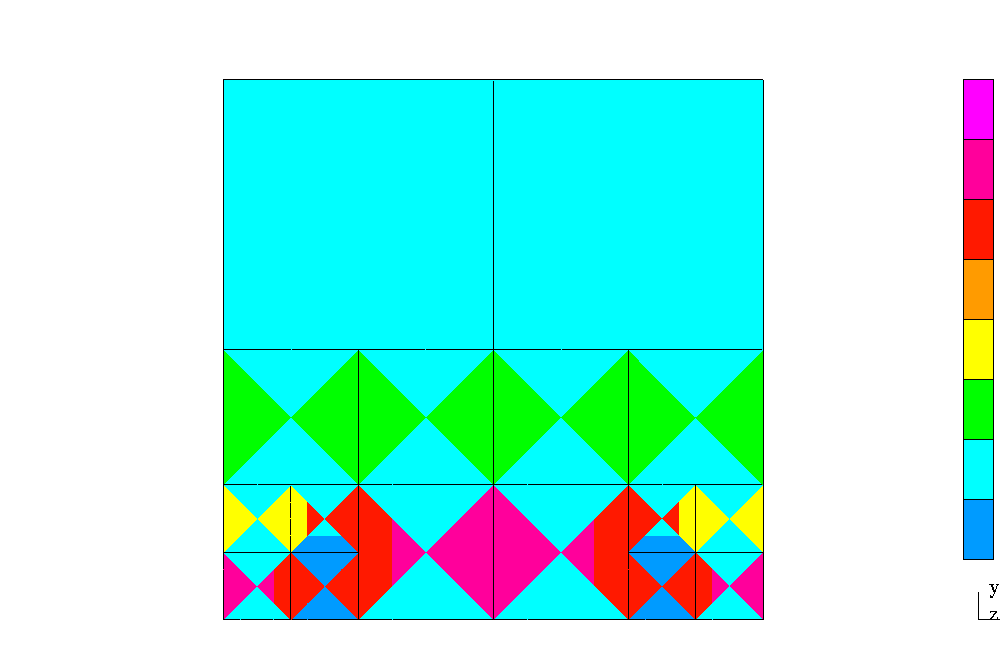
\includegraphics[scale=.2]{figs/mesh1.png}}
\subfigure{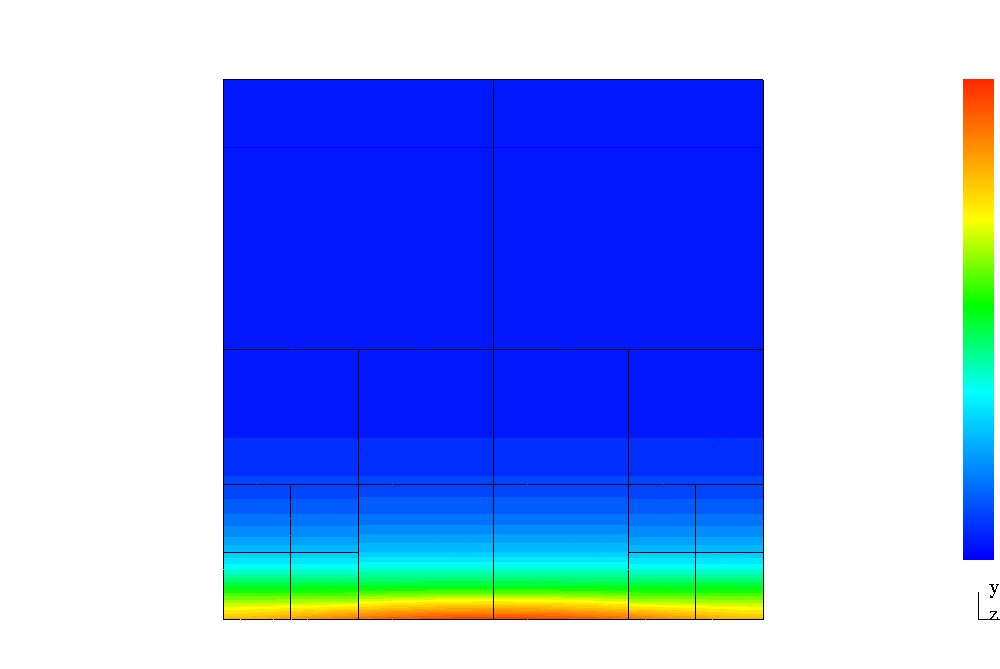
\includegraphics[scale=.2]{figs/sol1.png}}
\caption{The $v$ component of the optimal test function corresponding to flux $\widehat{u} = x(1-x)$ on the bottom side of a unit element for $\epsilon = 0.01$. The corresponding $hp$-mesh used to compute the solution is displayed to the left.}
\label{fig:boundaryTest}
\end{figure}
To avoid boundary layers in the optimal test functions, we follow \cite{DPGrobustness} in scaling the $L^2$ contributions of $v$ by $C_v(K)$, such that, when transformed to the reference element, both $C_v(K)\|v\|^2$ and $\epsilon\|\grad v\|^2$ are of the same magnitude. Similarly, we scale the $L^2$ contributions of $\tau$ by $C_\tau(K)$ such that $\frac{C_\tau(K)}{\epsilon} \|\tau\|^2$ and $\|\div \tau\|^2$ are of the same magnitude as well. For this work, we consider only isotropic refinements on quadrilateral elements in 2D.

Our test norm, as defined over a single element $K$, is now
\[
\|\left(v,\tau\right)\|_{V,K}^2 = \min\left\{\frac{\epsilon}{|K|},1\right\}\|v\|^2 + \epsilon \|\grad v\|^2 + \|\beta \cdot \grad v\|^2 + \| \div \tau\|^2 + \min\left\{\frac{1}{\epsilon},\frac{1}{|K|}\right\}\|\tau\|^2.
\]
This modified test norm avoids boundary layers in the locally computed optimal test functions, but for adaptive meshes, provides additional stability in areas of heavy refinement, where the best approximation error tends to be large and stronger robustness is most necessary.  This leads to a test norm which produces easily approximable optimal test functions, but still provides \textit{asymptotically} the strongest test norm and tightest robustness results in the areas of highest error. 

\subsubsection{Equivalence of energy norm with $\nor{\cdot}_U$}
%\subsection{Relations between trial and test constants}
\label{sec:main_bounds}

The main theoretical result of this work can now be given:
\begin{lemma}
Under the mesh-dependent test norm
\[
\|\left(v,\tau\right)\|_{V,\Oh}^2 = \|C_vv\|^2 + \epsilon \|\grad v\|^2 + \|\beta \cdot \grad v\|^2 + \| \div \tau\|^2 + \|C_\tau\tau\|^2,
\]
where $C_v, C_{\tau}\in L^2(\Omega)$ are defined elementwise through
\begin{align*}
\left.C_v\right |_K &= \min\left\{\sqrt{\frac{\epsilon}{|K|}},1\right\}\\
\left.C_{\tau}\right |_K &= \min\left\{\frac{1}{\sqrt{\epsilon}},\frac{1}{\sqrt{|K|}}\right\}.
\end{align*}
If $\beta$ satisfies \eqref{a_req}, \eqref{b_req}, and \eqref{c_req}, the DPG energy norm $\nor{\cdot}_E$ satisfies the following equivalence relations
\begin{align*}
\nor{u}_{L^2} + \nor{\sigma}_{L^2} + \epsilon\nor{\widehat{u}} + \sqrt{\epsilon}\nor{\widehat{f}_n} 
&\lesssim \nor{\left(u,\sigma, \widehat{u},\widehat{f}_n\right)}_E \\ 
%\nor{\left(u,\sigma, \widehat{u},\widehat{f}_n\right)}_E &\lesssim \nor{u}_{L^2} + \nor{C_\sigma \sigma}_{L^2} + \frac{1}{\sqrt{\epsilon}} \left(\nor{\widehat{u}} + \nor{\widehat{f}_n}\right),
\nor{\left(u,\sigma, \widehat{u},\widehat{f}_n\right)}_E &\lesssim \nor{u}_{L^2} + \nor{\frac{1}{\epsilon C_\tau} \sigma}_{L^2} + \frac{1}{\sqrt{\epsilon}} \left(\nor{\widehat{u}} + \nor{\widehat{f}_n}\right).
\end{align*}
%where $C_\sigma \in L^2(\Omega)$ is defined elementwise through $\left.C_\sigma\right|_K  = \max\left\{ \frac{1}{\sqrt{\epsilon}} , \frac{\sqrt{|K|}}{\epsilon} \right\}$.
\end{lemma}

\begin{proof}
We begin by proving the bound from below. As a consequence of the duality of norms discussed in Section~\secref{energyPair}, we know that the norm $\left\| u \right\|_{U,1}$ is induced by a specific test norm $\| v  \|_{V,U,1}$.  To bound $\|\cdot\|_E$ robustly from above or below by a given norm $\left\| u \right\|_{U,2}$ on $U$ now only requires the robust bound in the opposite direction of $\| v \|_{V,U,1}$ by $\|v\|_{V,U,2}$. 

For $f$ and $g$ defined in \eqref{adjoint1} and \eqref{adjoint2},
\begin{align*}
f &= \epsilon^{-1}\tau + \grad v  \\
g &=\div \tau - \beta\cdot \grad v,
\end{align*} 
we can characterize the test norm for 
\[
\left\|\left(u,\sigma,\widehat{u},\widehat{f}_n\right)\right\|_{U,1}^2 = \|u\|^2 + \|\sigma\|^2 + \epsilon\|\widehat{u}\|^2+ \sqrt{\epsilon}\|\widehat{u}\|^2
\]
through the equivalence relation
\begin{align*}
\|\left(v,\tau\right)\|_{V,U,1} &\simeq \sup_{u,\sigma,\widehat{u},\widehat{f}_n}\frac{b\left(\left(u,\sigma,\widehat{u},\widehat{f}_n\right),\left(\tau,v\right)\right)}{\|u\| + \|\sigma\| + \epsilon\|\widehat{u}\|+ \sqrt{\epsilon}\|\widehat{u}\|}\\
& \simeq \|g\| + \|f\| + \frac{1}{\epsilon}\sup_{\widehat{u}\neq 0, \left.\widehat{u}\right|_{\Gamma_+} = 0} \frac{\langle \jump{\tau\cdot n}, \widehat{u}\rangle}{\|\widehat{u}\|} + \frac{1}{\sqrt{\epsilon}}\sup_{\widehat{f}_n\neq 0, \left.\widehat{f}_n\right|_{\Gamma_-}=0}\frac{\langle \widehat{f}_n, \jump{v}\rangle}{\|\widehat{f}\|},
\end{align*}
which, by definition of the boundary norms, is 
\[
\|\left(v,\tau\right)\|_{V,U,1} \simeq \|g\| + \|f\| + \frac{1}{\epsilon}\|\jump{\tau\cdot n}\| + \frac{1}{\sqrt{\epsilon}}\|\jump{v}\|.
\]
We wish to show the bound
\[
\nor{\left(v,\tau\right)}_{V,\Oh} \lesssim \|g\| + \|f\| + \frac{1}{\epsilon}\|\jump{\tau\cdot n}\| + \frac{1}{\sqrt{\epsilon}}\|\jump{v}\|.
\]
By noting that both 
\begin{align*}
\nor{C_vv_0} &\leq \nor{v_0},\\
\nor{C_\tau\tau_0} &\leq \frac{1}{\sqrt{\epsilon}}\nor{\tau_0},
\end{align*}
we have that $\nor{\left(v,\tau\right)}_{V,\Oh} \leq \nor{\left(v,\tau\right)}_{V}$, so it suffices to prove the bound for the mesh-independent test norm 
\[
\|\left(v,\tau\right)\|_{V}^2 = \|v\|^2 + \epsilon \|\grad v\|^2 + \|\beta \cdot \grad v\|^2 + \| \div \tau\|^2 + \frac{1}{\epsilon}\|\tau\|^2.
\]

We will bound $\|\left(v,\tau\right)\|_V$ for all $\left(v,\tau\right)$ by decomposing $\left(v,\tau\right) = \left(v_0,\tau_0\right) + \left(v_1,\tau_1\right) + \left(v_2,\tau_2\right)$ as described in Section~\ref{sec:strategy2}. 

By the triangle inequality, robustly bounding $\|\left(v,\tau\right)\|_V$ from above reduces to robustly bounding each component 
\[
\|\left(v_{0},\tau_{0}\right)\|_V, \|\left(v_{1},\tau_{1}\right)\|_V, \|\left(v_{2},\tau_{2}\right)\|_V \lesssim \|g\| + \|f\| + \frac{1}{\epsilon}\|\jump{\tau\cdot n}\| + \frac{1}{\sqrt{\epsilon}}\|\jump{v}\|.
\]

%Roughly speaking, Lemma \ref{lemma_grad} concerns the robust control of $u$ by the energy error; Lemmas \ref{lemma_stream} and \ref{lemma_boundary} concern the robust control of field variable $\sigma$ and flux/trace variables, respectively.  

\begin{itemize}
\item \textbf{Bound on $\|\left(v_{0},\tau_{0}\right)\|_V$}
 
Lemma \ref{lemma_boundary} gives control over $\sqrt{\epsilon}\|\grad v_0\| + \frac{1}{\epsilon}\|\tau_0\|$ through
\[
\|\grad v_0\| = \frac{1}{\epsilon}\|\tau_0\| \lesssim \frac{1}{\epsilon} \nor{\jump{\tau_0\cdot n}}_{\Gamma_h \setminus \Gamma_+} + \frac{1}{\sqrt{\epsilon}} \nor{\jump{v_0}}_{\Gamma_h^0 \cup \Gamma_+} = \frac{1}{\epsilon} \nor{ \jump{\tau\cdot n}}_{\Gamma_h \setminus \Gamma_+} + \frac{1}{\sqrt{\epsilon}} \nor{ \jump{v}}_{\Gamma_h^0 \cup \Gamma_+}.
\]
Lemma 4.2 of \cite{analysisDPG} gives us the Poincare inequality for discontinuous functions
\[
\|v_0\| \lesssim \|\grad v_0\| + \|\jump{v}\|.
\]
%Since $f=0$, by Lemma 2, $\|\beta\cdot \grad v_0\|  \lesssim \|g\| = 0$.  
Since $g = 0$, $\| \div \tau_0\| = \|\beta\cdot \grad v_0\|\lesssim \|\grad v_0\|$, which we now have control over as well.  

\item \textbf{Bound on $\|\left(v_{1},\tau_{1}\right)\|_V$}

With $f = 0$, Lemma \ref{lemma_stream} provides the bound
\[
\|\beta \cdot \grad v_1 \| \lesssim \| g\|.
\]
Noting that $\div \tau_1 = g+\beta\cdot \grad v_1$ gives $\|\div \tau_1 \| \lesssim \|g\|$ as well.  Lemma \ref{lemma_grad} gives
\[
\epsilon \|\grad v_1\|^2 + \|v_1\|^2 \lesssim \|g\|^2,
\]
and noting that $\epsilon^{-1/2}\tau_1 = \epsilon^{1/2}\grad v_1$ gives $\epsilon\|\grad v_1\|^2 = \epsilon^{-1}\|\tau_1\|^2 \lesssim \|g\|^2$ as well.

\item \textbf{Bound on $\|\left(v_{2},\tau_{2}\right)\|_V$}

Lemma \ref{lemma_grad} provides, for $\epsilon$ sufficiently small, 
\[
\epsilon \|\grad v_2\|^2 + \|v_2\|^2 \lesssim  \epsilon \| f\|^2 \leq \|f\|^2.
\]
We have $\epsilon^{-1}\tau_2 = f - \grad v_2$, so $\epsilon^{-1} \|\tau_2\| \lesssim \|f\| + \|\grad v_2\|$. Lemma~\ref{lemma_grad} implies $\|\grad v_2\|^2  \lesssim  \| f\|^2$, so for $\epsilon \leq 1$, we have $\epsilon^{-1/2}\|\tau_2\| \leq \epsilon^{-1}\|\tau_2\| \lesssim \|f\|$.  The remaining terms can be bounded by noting that, with $g = 0$, $\|\div \tau_2\| = \|\beta\cdot \grad v_2\| \lesssim \|\grad v_2\| \lesssim \|f\| $.
\end{itemize}

We have shown the robust bound of the norm $\|\cdot \|_{U,1}$ on $U$ by the energy norm; for a full equivalence statement, we require a bound from above on the energy norm by the norm $\|\cdot \|_{U,2}$ on $U$.  By the duality of the energy and test norm, this is equivalent to bounding the test norm from below by the test norm induced by $\|\cdot \|_{U,2}$. 
For a norm on $U$ of the form
\[
\left\|\left(u,\sigma,\widehat{u},\widehat{f}_n\right)\right\|_{U,2}^2 = \|u\|^2 + \nor{C_\sigma \sigma}^2 + \frac{1}{{\epsilon}}\left( \|\widehat{u}\|^2 + \|\widehat{f}_n\|^2\right),
\]
the induced test norm is equivalent to
\begin{align*}
\| \left(\tau,v\right) \|_{V,U,2} &\simeq \sup_{\left(u,\sigma,\widehat{u},\widehat{f}_n\right) \in U\setminus \{0\}} \frac{b\left(\left(u,\sigma,\widehat{u},\widehat{f}_n\right),\left(\tau,v\right)\right)}{\left\|\left(u,\sigma,\widehat{u},\widehat{f}_n\right)\right\|_E} \\
&\simeq \sup_{\left(u,\sigma,\widehat{u},\widehat{f}_n\right) \in U\setminus \{0\}} \frac{\left(u,\div \tau - \beta \cdot \grad v\right) + \left(\sigma, \epsilon^{-1} \tau + \grad v\right) - \langle \jump{\tau_n}, \widehat{u} \rangle + \langle \widehat{f}_n, \jump{v} \rangle
}{\|u\| + \nor{\left(\epsilon C_\tau\right)^{-1}\sigma} + \frac{1}{\sqrt{\epsilon}}\left(  \|\widehat{u}\| + \|\widehat{f}_n\| \right)} \\
&\simeq \|g\| + \nor{\epsilon C_\tau f} + {\sqrt{\epsilon}}\left(\sup_{\widehat{u},\widehat{f}_n \neq 0}\frac{\langle \jump{\tau_n}, \widehat{u} \rangle + \langle \widehat{f}_n, \jump{v} \rangle}{\|\widehat{u}\| + \|\widehat{f}_n\|}\right),
\end{align*}
where $f$ and $g$ are 
\begin{align*}
f &= \frac{1}{\epsilon}\tau + \grad v\\
g &= \div \tau - \beta \cdot \grad v,
\end{align*}
the loads of the adjoint problem defined in \eqref{adjoint1}, \eqref{adjoint2}.  

Note that $\epsilon C_\tau \leq \sqrt{\epsilon}$. Then, by the triangle inequality, we have the bounds
\begin{align*}
%\sqrt{\epsilon} \|f \| &\leq \epsilon^{-1/2} \| \tau\| + \sqrt{\epsilon} \|\grad v\| \lesssim \|\\
\|\epsilon C_\tau f \| &\leq C_\tau \nor{ \tau} + \epsilon C_\tau \nor{\grad v} \lesssim \| \left(\tau,v\right)\|_{V,\Oh}\\
\|g \| &\leq \|\div \tau\| +  \|\beta \cdot \grad v\| \lesssim \| \left(\tau,v\right)\|_{V,\Oh}
\end{align*}
We estimate the supremum on the jumps of $\left(\tau,v\right)$ by following \cite{DPGrobustness}; we begin by choosing $\eta \in H({\rm div}; \Omega)$, $w\in H^1(\Omega)$, such that $\left.\left(\eta-\beta w \right)\cdot n\right |_{\Gamma_+} = 0$ and $\left.w\right |_{\Gamma_-\cup\Gamma_0} = 0$, and integrating the boundary pairing by parts to get
\begin{align*}
\langle \jump{\tau\cdot n},w\rangle + \langle \jump{v},\left(\eta - \beta w\right)\cdot n\rangle &= (\tau,\grad w) + (\div \tau, w) + \left(\eta - \beta w, \grad v\right) +  \left(\div \left(\eta - \beta w\right), v\right)\\
&\lesssim \|C_\tau\tau\| \nor{ \frac{1}{C_\tau}\grad w} + \|\div \tau\| \|w\| \\
&\left.\hspace{.3cm}\right. + \sqrt{\epsilon}\| \grad v \|\frac{1}{\sqrt{\epsilon}}\|\eta\| +  \|\beta \cdot \grad v\| \| w\|\\
&\left.\hspace{.3cm}\right. + \|C_vv\|\nor{\frac{1}{C_v}\div \eta} + \| C_vv\| \nor{\frac{1}{C_v}w} \\
&\left.\hspace{.3cm}\right. + \|C_v v\| \nor{\frac{1}{C_v} \grad w},
\end{align*}
where we have used that $\epsilon < 1$, $\div \beta = O(1)$, and that $\|\beta\cdot \grad w\|\lesssim \|\grad w\|$.  

Without loss of generality, assume the problem is scaled such that $\max_{K\in\Oh}|K| \leq 1$. Then, $\frac{1}{C_\tau^2}\leq \frac{1}{C_v^2} \leq \frac{1}{\epsilon}$, and an application of discrete Cauchy-Schwarz gives us 
\begin{align*}
\langle \jump{\tau\cdot n},w\rangle + \langle \jump{v},\left(\eta - \beta w\right)\cdot n\rangle &\lesssim \|\left(\tau,v\right)\|_{V,\Oh}\frac{1}{\sqrt{\epsilon}}\left(\nor{\eta}_{H({\rm div},\Omega)} + \nor{w}_{H^1(\Omega)}\right),\\
&\lesssim \|\left(\tau,v\right)\|_{V,\Oh}\frac{1}{\sqrt{\epsilon}}\left(\nor{\eta-\beta w}_{H({\rm div},\Omega)} + \nor{w}_{H^1(\Omega)}\right),
\end{align*}
since $\|\eta\|_{H({\rm div},\Omega)} = \|\eta - \beta w + \beta w\|_{H({\rm div},\Omega)} \leq \|\eta - \beta w\|_{H({\rm div},\Omega)} + \|\beta w\|_{H({\rm div},\Omega)} \lesssim \|\eta-\beta w\|_{H({\rm div},\Omega)} + \|w\|_{H^1(\Omega)}$.  Dividing through and taking the supremum gives
\[
\sup_{w,\eta \neq 0} \frac{\langle\jump{\tau\cdot n},w\rangle + \langle \jump{v},\left(\eta - \beta w\right)\cdot n\rangle}{\left(\nor{\eta-\beta w}_{H({\rm div},\Omega)} + \nor{w}_{H^1(\Omega)}\right)} \lesssim \|\left(\tau,v\right)\|_{V,\Oh}\frac{1}{\sqrt{\epsilon}}.
\]
To finish the proof, define $\rho \in H^{1/2}(\Gamma_h)$ and $\phi \in H^{-1/2}(\Gamma_h)$ such that $\rho = \left.w\right|_{\Gamma_h}$ and $\phi = \left.(\eta-\beta w)\cdot n\right|_{\Gamma_h}$, and note that, from \cite{analysisDPG}, by the definition of the trace norms on $\jump{\tau\cdot n}$ and $\jump{v}$ 
\begin{align*}
\sup_{\rho,\phi \neq 0} \frac{\langle \jump{\tau\cdot n},\rho\rangle + \langle \jump{v},\phi \rangle}{\|\rho\|_{H^{1/2}(\Gamma_h)}+\|\phi\|_{H^{-1/2}(\Gamma_h)}} &= \sup_{w,\eta \neq 0} \frac{\langle \jump{\tau\cdot n},w\rangle + \langle \jump{v},\left(\eta - \beta w\right)\cdot n\rangle}{ \|w\|_{H^1(\Omega)}+\|\eta-\beta w\|_{H({\rm div},\Omega)}}.
\end{align*}
Together, the bounds on the jump terms and the bounds on $\|g\|$ and $\|f\|$ imply $\left\|\left(u,\sigma,\widehat{u},\widehat{f}_n\right)\right\|_{E} \lesssim \left\|\left(u,\sigma,\widehat{u},\widehat{f}_n\right)\right\|_{U,2}$.
\end{proof}

\subsubsection{Comparison of boundary conditions}

It is worth addressing the effect of boundary conditions on stability.  Specifically, a test norm that provides stability for one set of boundary conditions may perform poorly for another set.  Take, for example, the test norm defined in Section~\ref{sec:main_bounds} and the convection-diffusion problem with Dirichlet boundary conditions. 

The bilinear form for the case of Dirichlet boundary conditions is 
\[
b\left(\left(u,\sigma, \widehat{u}, \widehat{\sigma}_n\right), \left(v,\tau\right)\right) = \left(u,\div \tau - \beta \cdot \grad v\right) + \left(\sigma, \epsilon^{-1} \tau + \grad v\right) + \langle \widehat{u}, \jump{\tau \cdot n} \rangle_{\Gh^0} + \langle \widehat{f}_n, \jump{v} \rangle_{\Gh}.
\]
Notice that the boundary terms in the final bilinear form are different; hence, the adjoint problems associated with Section~\ref{sec:strategy3} will now carry different boundary conditions as well. Likewise, the stability properties proven previously will not hold under a different set of boundary conditions.  
%We note that 
%\begin{align*}
%b\left(\left(u,\sigma, \widehat{u}, \widehat{\sigma}_n\right), \left(\tau, v\right)\right) &= \left(u,\div \tau - \beta \cdot \grad v\right) + \left(\sigma, \epsilon^{-1} \tau + \grad v\right) - \langle \left[\tau_n\right], \widehat{u} \rangle_{\Gh^0} + \langle \widehat{f}_n, \left[v\right] \rangle_{\Gh} 
%&= \| u \|^2_{L^2}
%\end{align*}
%for the specific continuous test functions $\tau$ and $v$ satisfying
%\begin{align*}
%\div \tau - \beta \cdot \grad v &= u \\
%\frac{1}{\epsilon}\tau + \grad v &= 0
%\end{align*}
%with boundary condition $\left.v\right|_\Gamma = 0$. Choosing a continuous conforming test function $v$ removes the contribution of the term $\langle \widehat{f}_n, \left[v\right] \rangle$ on the mesh skeleton, while the boundary conditions remove the contribution of boundary terms from the bilinear form.  Then, for this specific choice of $\left(\tau, v\right)$, 
%\begin{align*}
%\|u\|_{L^2}^2 &= b\left(\left(u,\sigma, \widehat{u}, \widehat{\sigma}_n\right), \left(\tau, v\right)\right) = \frac{b\left(\left(u,\sigma, \widehat{u}, \widehat{\sigma}_n\right), \left(\tau, v\right)\right)}{\|\left(\tau, v\right)\|_V}\|\left(\tau, v\right)\|_V \leq \|u\|_E \|\left(\tau, v\right)\|_V
%\end{align*}
%At minimum, we want $\|u\|_{L^2} \lesssim \|u\|_E$, which requires 
%\[
%\|\left(\tau, v\right)\|_V \lesssim \| u \|_{L^2}
%\]
%for any choice of $u \in L^2$ (dividing through by $\|u\|_{L^2}$ gives the desired result).  This can be considered a ``sanity check"; at the minimum, we at least want control over the behavior of the single field variable $u$.  However, we are unable to prove this in the case of Dirichlet boundary conditions. 

As it turns out, the robust bounds given in Section~\ref{sec:main_bounds} hold in $\mathbb{R}^d$ for arbitrary $d$; however, we can show that for the case of Dirichlet boundary conditions, the same results do not hold, even in 1D.  
%In 1D, the problem reduces to 
%\begin{align*}
%\frac{1}{\epsilon}\sigma - u' &= 0\\
%\left(u - \epsilon \sigma \right)' &=f
%\end{align*}
%with bilinear form
%\begin{align*}
%b\left(\left(u,\sigma,\widehat{u},\widehat{f}\right),\left(\tau,v\right)\right) &= \sum_{k=1}^N \left(\left.\widehat{u}(x) \tau(x)\right |^{x_k}_{x_{k-1}} + \left.\widehat{f}(x) v(x)\right |^{x_k}_{x_{k-1}}\right) \\
%&+ \left(\sigma,\epsilon^{-1}\tau\right)_{\Oh} + (u,\tau')_{\Oh}- \left(u - \epsilon \sigma,v'\right)_{\Oh}
%\end{align*}
%where $\widehat{u}(x), \widehat{f}(x) \in \mathbb{R}$ are now point values defined on mesh points $x_k$ for $k=1,\ldots,N$, where $N$ is the number of elements.  We can assume without loss of generality that $\Oh$ is the unit interval $(0,1)$.  
%
%Let us first provide an interpretation of Lemma~\ref{lemma_stream}. Recall the bilinear form 
%\begin{align*}
%b\left(\left(u,\sigma, \widehat{u}, \widehat{f}_n\right),
%\left( v, \tau \right)\right) = \left(u,\div \tau - \beta \cdot \grad
%v\right)_{\Oh} + \left(\sigma, \epsilon^{-1} \tau + \grad v\right)_{\Oh} - \LRa{
%\jump{\tau\cdot n}, \widehat{u} }_{\Gh} + \LRa{ \widehat{f}_n,
%  \jump{v} }_{\Gh},
%\end{align*}
%By choosing $(v,\tau)$ such that
%\begin{align*}
%\div \tau - \beta \cdot \grad v &= u \\
%\frac{1}{\epsilon} \tau + \grad v &= 0
%\end{align*}
%we will have 
%\[
%b\left(\left(u,\sigma, \widehat{u}, \widehat{f}_n\right),
%\left( v, \tau \right)\right) =\|u\|_{L^2}^2 
%\]
%Given this, we can use the definition of the energy norm \eqnref{energyNorm} to bound
%\[
%\|u\|_{L^2}^2 = b\left(\left(u,\sigma, \widehat{u}, \widehat{f}_n\right),
%\left( v, \tau \right)\right) = \frac{b\left(\left(u,\sigma, \widehat{u}, \widehat{f}_n\right),
%\left( v, \tau \right)\right)}{\|(v,\tau)\|_V}\|(v,\tau)\|_V \lesssim \|u\|_E \|(v,\tau)\|_V
%\]
%If we can show that $\|(v,\tau)\|_V \lesssim \|u\|_{L^2}$ for $(v,\tau)$ as defined above, then this implies 
%\[
%\|u\|_{L^2} \lesssim \|u\|_E
%\]
%By the fact that 
Consider now the 1D analogue of the estimate given by Lemma~\ref{lemma_stream}.  In 1D, $\|\beta\cdot\grad v_1\| \lesssim \|g\|$ reduces to the inequality 
\[
\|\beta v_1'\|\lesssim \|g\|, \quad g\in L^2\!\left(\Oh\right).
\]
Without this inequality, we are unable to prove the robust bound on the $L^2$ error $\|u-u_h\|_{L^2} \lesssim \nor{(u,\sigma,\widehat{u},\widehat{f}_n)-(u_h,\sigma_h,\widehat{u}_h,\widehat{f}_{n,h})}_E$.

The adjoint problem corresponding to Lemma~\ref{lemma_stream} in Section~\ref{sec:strategy3} is likewise reduced in 1D to the scalar equation
\begin{align}
\epsilon v_1'' + \beta v_1' &= -g \label{adjoint_1D}
\end{align}
with $v_1\in H^1_0\left((0,1)\right)$.  After multiplying this equation by $\beta v_1'$ and integrate by parts over $\Oh$, we can apply Young's inequality to get
%\[
%\int_0^1 \epsilon v_1'' \beta v_1' + \|\beta v_1'\|_{L^2}^2 = -\int_0^1 g \beta v_1'.\
%]
%Integrating by parts and Young's inequality gives
\begin{align*}
\left.\frac{\epsilon}{2} \beta v_1'^2\right|_0^1 + \|\beta v_1'\|_{L^2}^2 &\leq \frac{1}{2}\|g\|^2 + \frac{1}{2}\|\beta v_1'\|^2,
\end{align*}
implying that
\begin{align*}
\|\beta v_1'\|_{L^2}^2 & \lesssim \|g\|^2 + {\beta \epsilon} v_1'(0)^2.
\end{align*}
Let us restrict ourselves to the cases where $v_1$ is sufficiently smooth for $v'(0)$ to be well defined.  Taking $g=1$ (corresponding to a piecewise constant approximation) we can solve \eqref{adjoint_1D} exactly. 
\begin{figure}[!h]
\centering
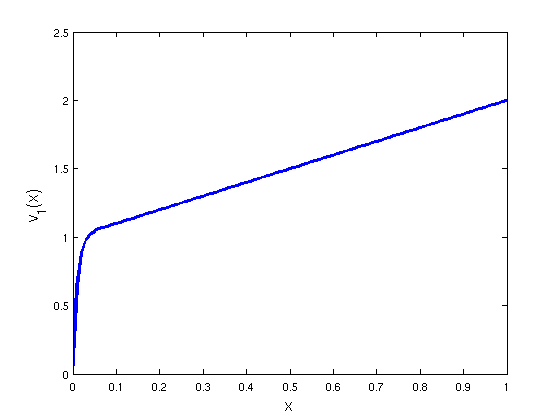
\includegraphics[scale=.5]{figs/testBoundary1D.png}
\caption{$v_1(x) = \frac{e^{-\frac{x}{\epsilon}}}{e^{\frac{1}{\epsilon}}-1}\left(e^{\frac{1}{\epsilon}}\left(e^{\frac{x}{\epsilon}}-1\right) + \left(e^{\frac{1}{\epsilon}}-1\right)e^{\frac{x}{\epsilon}}x\right)$, the solution to the adjoint equation for $f=0$ and constant $\beta$ and load $g$ for $\epsilon = .01$.}
\label{fig:testBoundary1D}
\end{figure}
The solution $v_1$ is plotted in Figure~\ref{fig:testBoundary1D}, where we can see that $v_1(x)$ develops strong boundary layers of width $\epsilon$ near the inflow boundary $x=0$. Consequently, $\frac{\epsilon}{2} v_1'(0)^2 \approx \epsilon^{-1}$. Thus, we cannot conclude $\|\beta v'\| \lesssim \|g\|$ when $g$ is a constant,\footnote{Unlike the case of Dirichlet boundary conditions, the inflow condition on $ \widehat{f}_n = u(0)-\epsilon u'(0)$ induces an adjoint boundary condition $\tau(0)=0$, or equivalently $v'(0) = 0$, removing the non-robust term from the estimate.} and as a consequence cannot conclude that the robust error bound $\|u-u_h\|_{L^2} \lesssim \|(u,\sigma,\widehat{u},\widehat{f}_n)-(u_h,\sigma_h,\widehat{u}_h,\widehat{f}_{n,h})\|_E$ holds for the solution $u_h$.  More detailed 1D error bounds for Dirichlet boundary conditions are provided in \cite{DPG3}, and indicate the same lack of robustness under the test norm used thus far.\footnote{Demkowicz and Heuer proved in \cite{DPGrobustness} that for Dirichlet boundary conditions, robustness as $\epsilon \rightarrow 0$ is achieved by the test norm
\[
\|\left(\tau, v\right)\|_{V,w}^2 = \|v\| + \epsilon \|\grad v\| + \|\beta \cdot \grad v\|_{w+\epsilon} + \| \div \tau\|_{w+\epsilon} + \frac{1}{\epsilon}\|\tau\|_{w+\epsilon}
\]
where $\|\cdot \|_{w+\epsilon}$ is a weighted $L^2$ norm, where the weight $w \in (0,1)$ is required to vanish on $\Gamma_-$ and satisfy $\grad w = O(1)$. The need for this weight is necessary to account for the loss of robustness at the inflow.} 

\begin{figure}[h!]
\centering
\subfigure[Primal problem, Dirichlet inflow BC]{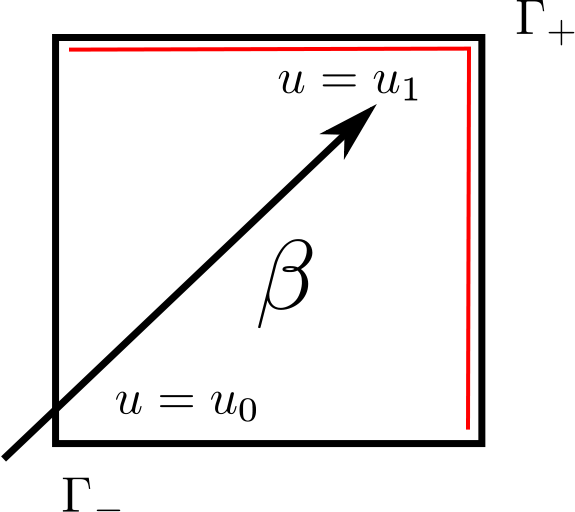
\includegraphics[scale=.3]{figs/primalDir.png}}
\subfigure[Adjoint problem, Dirichlet inflow BC]{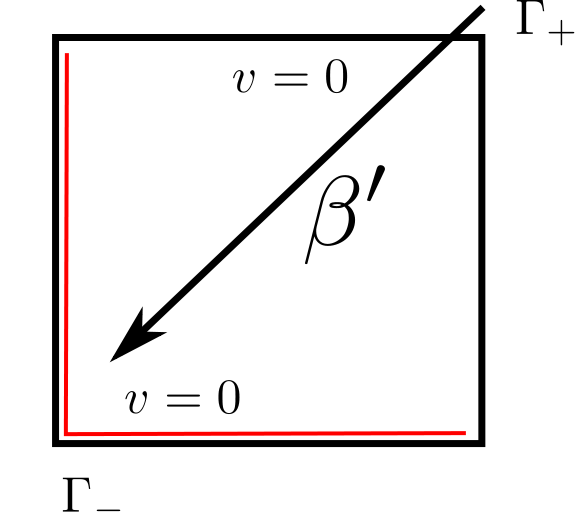
\includegraphics[scale=.3]{figs/adjointDir.png}}
\subfigure[Primal problem, new inflow BC]{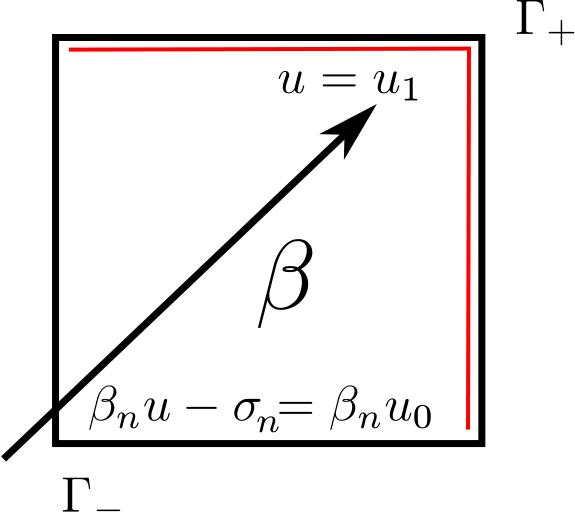
\includegraphics[scale=.3]{figs/primal.png}}
\subfigure[Adjoint problem, new inflow BC]{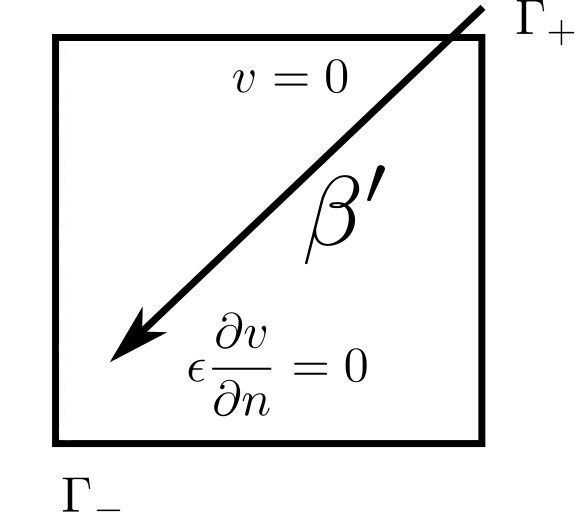
\includegraphics[scale=.3]{figs/adjoint.png}}
\caption{Comparison of primal and adjoint problems under both the standard Dirichlet and the new inflow boundary condition. The outflow boundary for each problem is denoted in red. For the standard Dirichlet inflow condition, the solution to the adjoint problem can develop strong boundary layers at the outflow of the adjoint problem. Notice, under the new inflow conditions, the relaxation of a wall-stop boundary condition with a zero-stress condition at the outflow boundary of the adjoint problem.}
\end{figure}

In higher dimensions, the adjoint problem is of the same form as the primal problem with the direction of convection reversed. However, the primal problem determines adjoint boundary conditions on $\Gamma_-$ and $\Gamma_+$. Thus, wheareas for the primal problem, data is convected from the inflow to the outflow, in the adjoint problem, data is convected from the outflow to the inflow boundary instead. 

We can intuitively explain the loss of robustness under our derived test norm by the presence of the Dirichlet boundary condition on $v$ at the inflow boundary. Since the direction of convection is reversed in the adjoint equation, we can interpret the adjoint as representing the convection of a concentration $v$ from the outflow to the inflow boundary. In the presence of a Dirichlet boundary condition at the inflow, $v$ can develop strong boundary layers at the inflow. As a consequence, the quantities $\|\beta\cdot \grad v\|$ and $\sqrt{\epsilon}\|\grad v\|$ are no longer robustly bounded by $\|f\|$ and $\|g\|$, and we can no longer derive robust bounds on the error $\|u-u_h\|_{L^2}$ by the error in the energy norm.

Recall our strategy for analysis was to decompose of $(v,\tau)$ into continuous and discontinuous portions. Mathematically speaking, the use of Dirichlet boundary conditions on the primal problem introduces strong boundary layers into the solution $v$ of the adjoint equation --- in other words, boundary layers are introduced into the continuous portions of our decomposition of $(v,\tau)$.\footnote{The boundary conditions do not introduce boundary layers into the actual computed test functions. However, an interesting phenomenon observed is that, for small $\epsilon$, a lack of robustness can manifest itself during numerical experiments as additional refinements near the inflow boundary, precisely where the continuous parts of the decomposition of $(v,\tau)$ develop boundary layers.} The new inflow boundary condition on the primal problem relaxes the wall boundary condition induced on the adjoint/dual problem with a boundary condition that does not generate boundary layers, resulting in stronger stability estimates for the adjoint, and a better result for the primal problem. 

%\begin{figure}[h]
%\centering
%\subfigure[Primal problem]{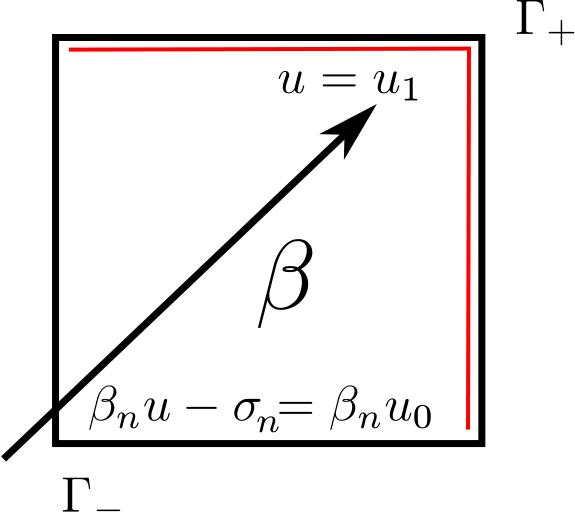
\includegraphics[scale=.3]{figs/primal.png}}
%\subfigure[Adjoint problem]{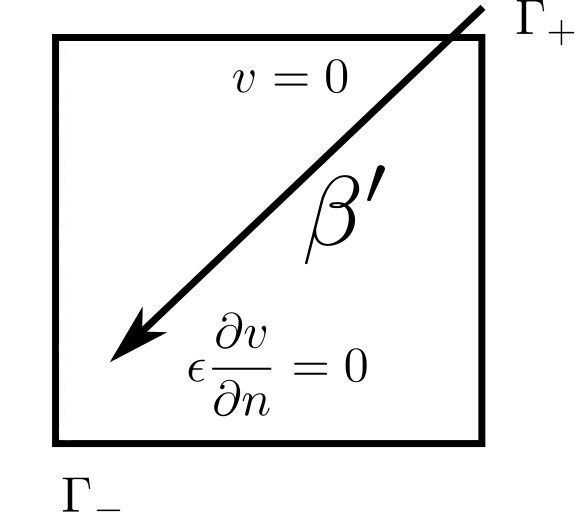
\includegraphics[scale=.3]{figs/adjoint.png}}
%\caption{Comparison of primal and adjoint problems for convection-diffusion under the standard Dirichlet outflow boundary condition and the new inflow boundary condition. Notice the replacement of a wall-stop boundary condition with a Neumann stress boundary condition at the outflow boundary of the adjoint problem. }
%\end{figure}

\section{Numerical experiments: Eriksson-Johnson problem}
\label{sec:num_exp}

In each numerical experiment, we vary $\epsilon = .01, .001, .0001$ in order to demonstrate robustness over a range of $\epsilon$.  This is intended to mirror the experience with roundoff effects in numerical experiments \cite{DPGrobustness}; for ``worst-case" linear solvers, such as LU decomposition without pivoting, the effect of roundoff error becomes evident in the solving of optimal test functions for $\epsilon \leq O(1e-5)$.  The roundoff itself comes from the conditioning of the Gram matrix under certain test norms; for example, if the weighted $H({\rm div};\Omega)\times H^1(\Omega)$ norm is used for the test norm $\|\left(\tau,v\right)\|_V$ (as was done in \cite{DPG2}), for an element of size $h$, $\|v\|_{L^2}^2 = O(h)$, while $\|\grad v\|_{L^2}^2 = O(h^{-1})$. As $h\rightarrow 0$, the seminorm portion of the test norm dominates the Gram matrix, leading to a near-singular and ill-conditioned system. 

The effect of roundoff error is often characterized by an increase in the energy error, which (assuming negligible error in the approximation of test functions) is proven to decrease for any series of refined meshes. These roundoff effects are dependent primarily on the mesh, appearing when trying to fully resolve very thin boundary layers by introducing elements of size $\epsilon$ through adaptivity. The effects of roundoff error were successfully treated in \cite{DPG3} by dynamically rescaling the test norms based on element size, a practical remedy not covered yet by the present analysis. 

To confirm our theoretical results, we adopt a modification of a problem first proposed by Eriksson and Johnson in \cite{Eriksson1993}. For the choice of $\Omega = (0,1)^2$, $f=0$, and $\beta = (1,0)^T$, the convection diffusion equation reduces to
\[
\pd{u}{x} - \epsilon \left(\pdd{u}{x}+ \pdd{u}{y}\right) = 0,
\]
which has an exact solution by separation of variables, allowing us to analyze convergence of DPG for a wide range of $\epsilon$.  For boundary conditions, we impose $u=0$ on $\Gamma_+$ and $\beta_n u - \sigma_n$ on $\Gamma_-$, which reduces to
\begin{align*}
u-\sigma_x &= u_0-\sigma_{x,0}, \quad x=0,\\
\sigma_y &=  0, \quad y=0,1,\\
u &= 0, \quad x=1.\\
\end{align*}
In this case, our exact solution is the series
\[
u(x,y) = C_0 + \sum_{n=1}^\infty C_n \frac{\exp(r_2(x-1)-\exp(r_1(x-1)))}{r_1\exp(-r2) - r_2\exp(-r1)}\cos(n\pi y),
\]
where
\begin{align*}
r_{1,2} &= \frac{1 \pm \sqrt{1 + 4 \epsilon\lambda_n}}{2 \epsilon},\\
\lambda_n &= n^2\pi^2 \epsilon.
\end{align*}
The constants $C_n$ depend on a given inflow condition $u_0$ at $x=0$ via the formula
\[
C_n = \int_0^1 u_0(y) \cos(n\pi y).
\]

All computations have been done using the adaptive DPG code Camellia, built on the Sandia toolbox Trilinos \cite{Camellia}.

\subsection{Solution with $C_1 = 1, C_{n\neq 1} = 0$}

We begin with the solution taken to be the first non-constant term of the above series.  We set the inflow boundary condition to be exactly the value of $u-\sigma_x$ corresponding to the exact solution.  

\begin{figure}[h!]
\centering
\subfigure{
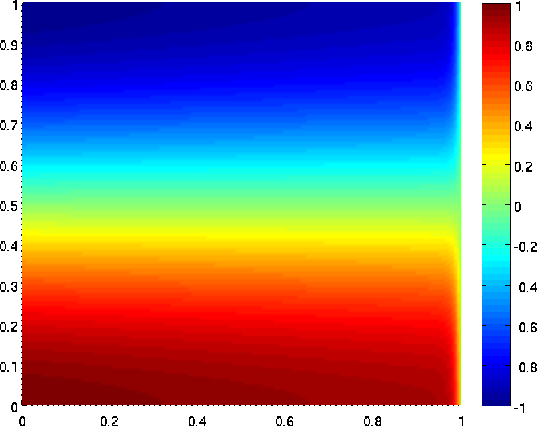
\includegraphics[scale=.37]{figs/wallBC_exact_u.png}
}
\subfigure{
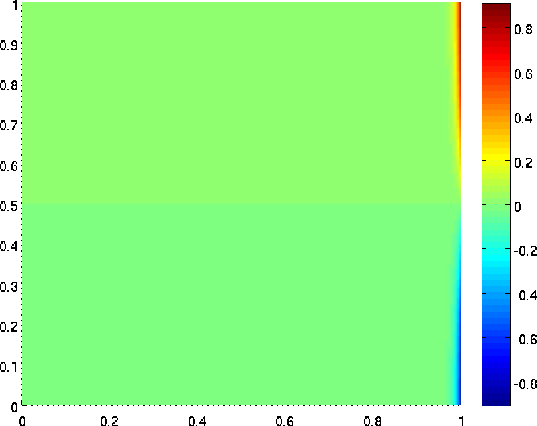
\includegraphics[scale=.37]{figs/wallBC_exact_sigx.png}
}
\subfigure{
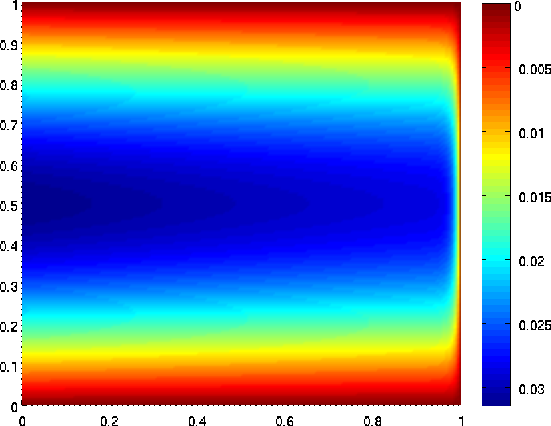
\includegraphics[scale=.37]{figs/wallBC_exact_sigy.png}
}
\caption{Solution for $u$, $\sigma_x$, and $\sigma_y$ for $\epsilon = .01$, $C_1 = 1$, $C_n=0$, $n\neq 1$}
\end{figure}
In each case, we begin with a square 4 by 4 mesh of quadrilateral elements with order $p=3$.  We choose $\Delta p = 5$, though we note that the behavior of DPG is nearly identical for any $\Delta p \leq 3$, and qualitatively the same for $\Delta p = 2$.  $h$-refinements are executed using a greedy refinement algorithm, where element energy error $e_K^2$ is computed for all elements $K$, and elements such that $e_K^2 \leq \alpha \max_K e_K^2$ are refined.  We make the arbitrary choice of taking $\alpha = .2$ for each of these experiments.  

\begin{figure}[h!]
\centering
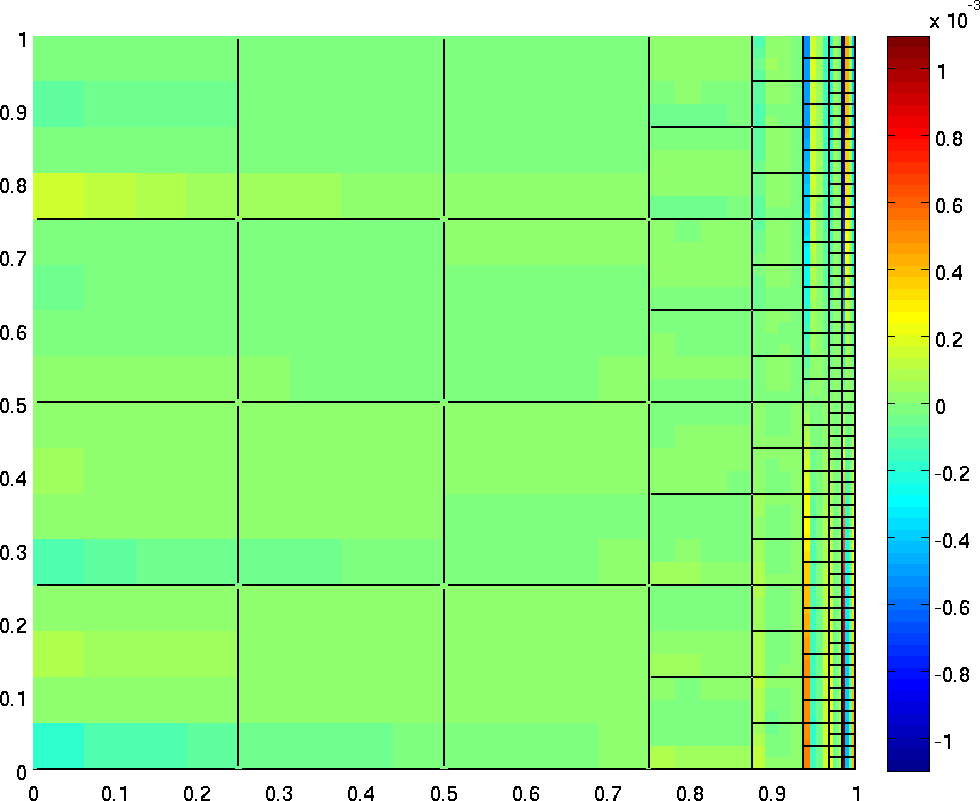
\includegraphics[scale=.4]{figs/u_pointdiff_wallBC.png}
\caption{Adapted mesh and pointwise error for $\epsilon=.01$}
\end{figure}
We are especially interested in the ratio of energy error and total $L^2$ error in both $\sigma$ and $u$, which we denote as $\|u-u_h\|_{L^2}$.  The bounds on $\nor{\cdot}_E$ presented in Section~\ref{sec:main_bounds} imply that, using the above test norm, $\|u-u_h\|_{L^2} / \|u-u_h\|_E \leq C$ independent of $\epsilon$.  Figure~\ref{ratios_simple}, which plots the ratio of $L^2$ to energy error, seems to imply that (at least for this model problem) $C=O(1)$.  Additionally, while we do not have a robust lower bound ($\|u-u_h\|_{L^2} / \|u-u_h\|_E$ can approach $0$ as $\epsilon \rightarrow 0$), our numerical results appear to indicate the existence of an $\epsilon$-independent lower bound. 

\begin{figure}[h!]
\centering
\subfigure{
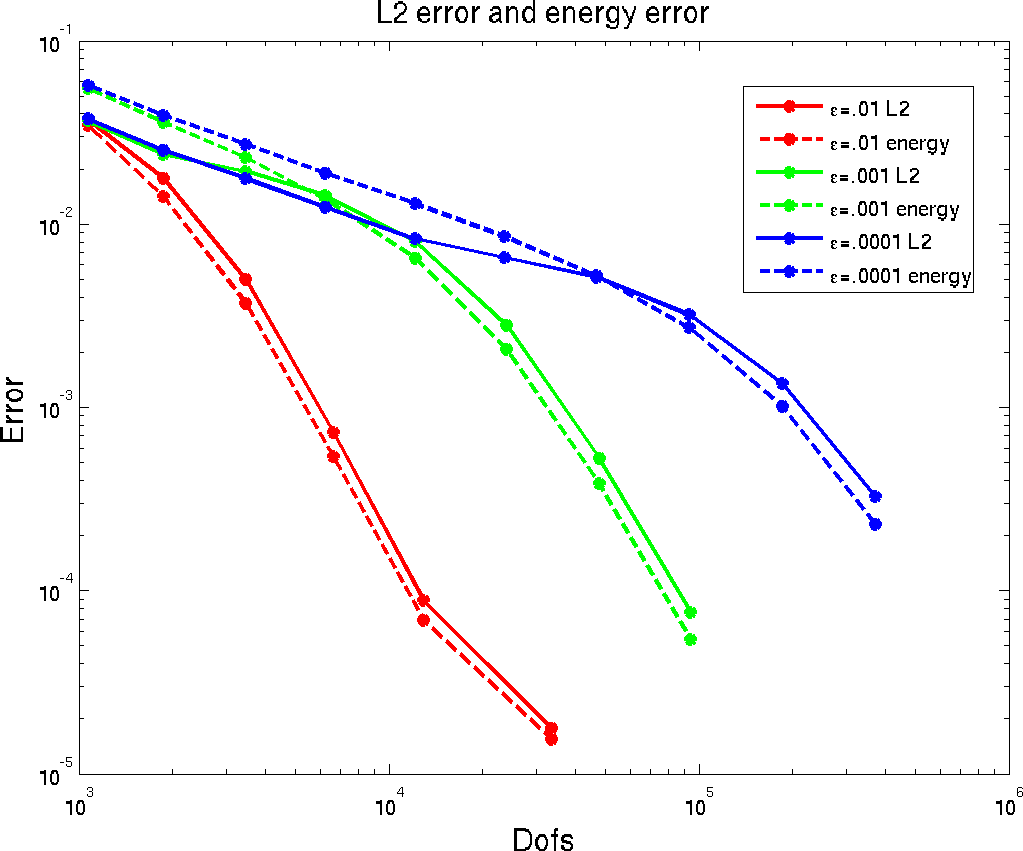
\includegraphics[scale=.38]{figs/errorrates_wallBC.png}
}
\subfigure{
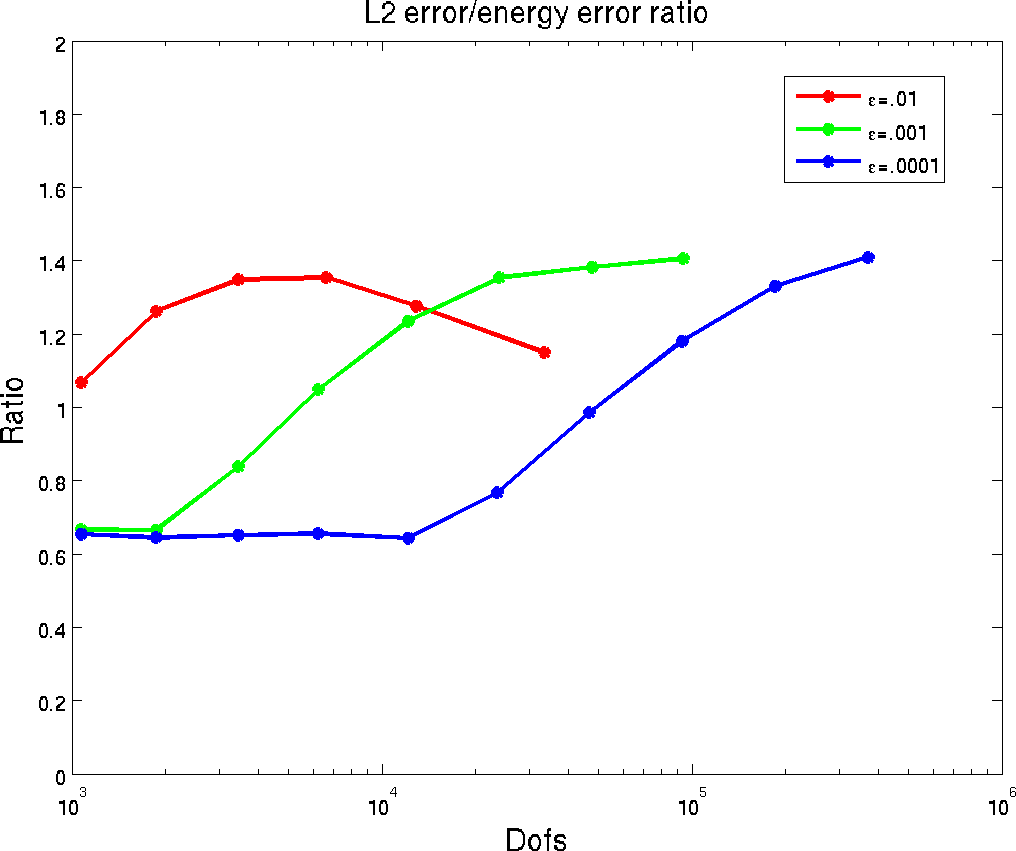
\includegraphics[scale=.38]{figs/L2energyratio_wallBC.png}
}
\caption{$L^2$ and energy errors, and their ratio for $\epsilon=.01$, $\epsilon=.001$, $\epsilon=.0001$}
\label{ratios_simple}
\end{figure}
The effect of a mesh dependent scalings on the $\|v\|^2$ and $\|\tau\|^2$ terms in the test norm can be seen in the ratios of $L^2$ to energy error; as the mesh is refined, the constants in front of the $L^2$ terms for $v$ and $\tau$ converge to stationary values (providing the full robustness implied by our adjoint energy estimates), and the ratio of $L^2$ to energy error transitions from a smaller to a larger value.  The transition point happens later for smaller $\epsilon$, which we expect, since the transition of the ratio corresponds to the introduction of elements whose size is of order $\epsilon$ through mesh refinement. 

We examined how small $\epsilon$ needed to be in order to encounter roundoff effects as well. In \cite{DPGrobustness}, the smallest resolvable $\epsilon$ using only double precision arithmetic was $1e-4$. The solution of optimal test functions is now done using both pivoting and equilibration, improving conditioning. Roundoff effects still appear, but at smaller values of $\epsilon$.

\begin{figure}[h!]
\centering
\subfigure{
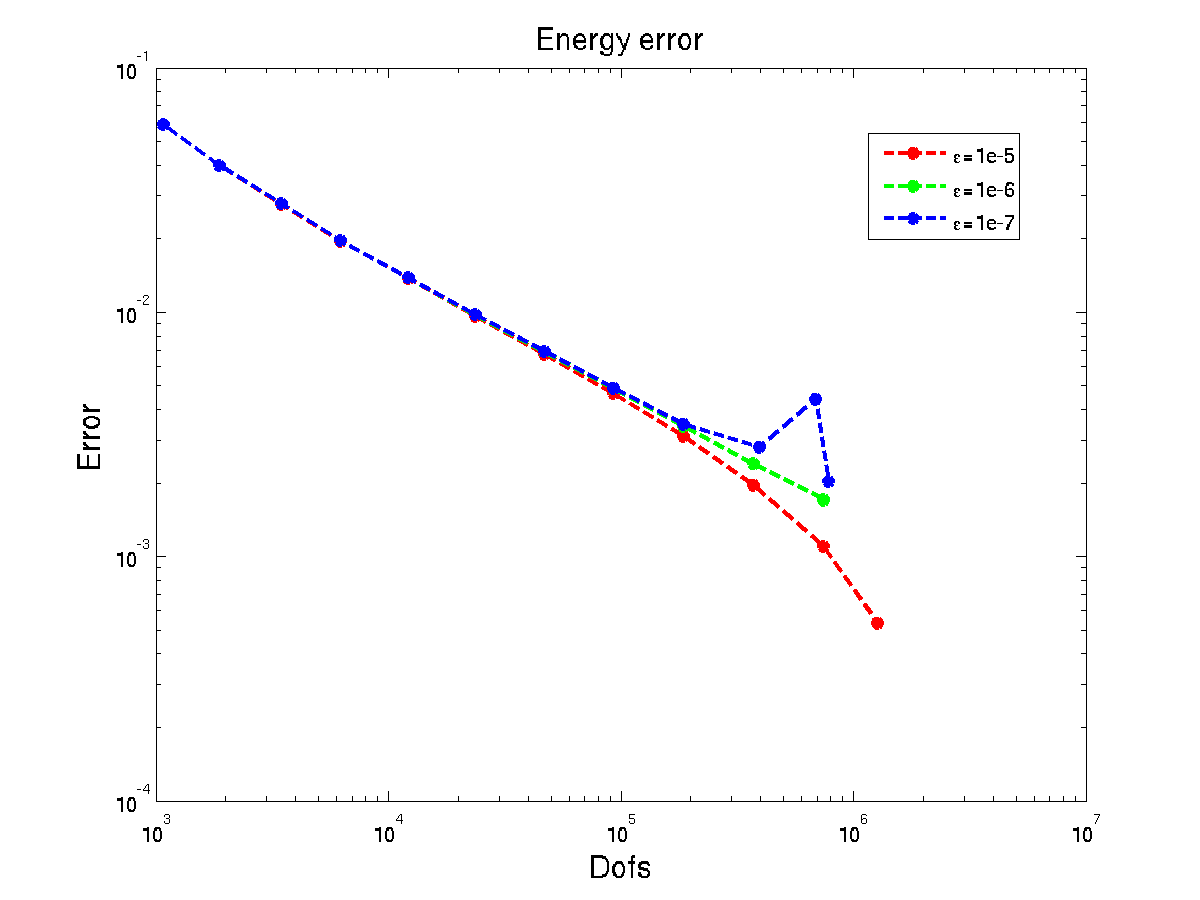
\includegraphics[scale=.36]{figs/roundoff_rates.png}
}
\subfigure{
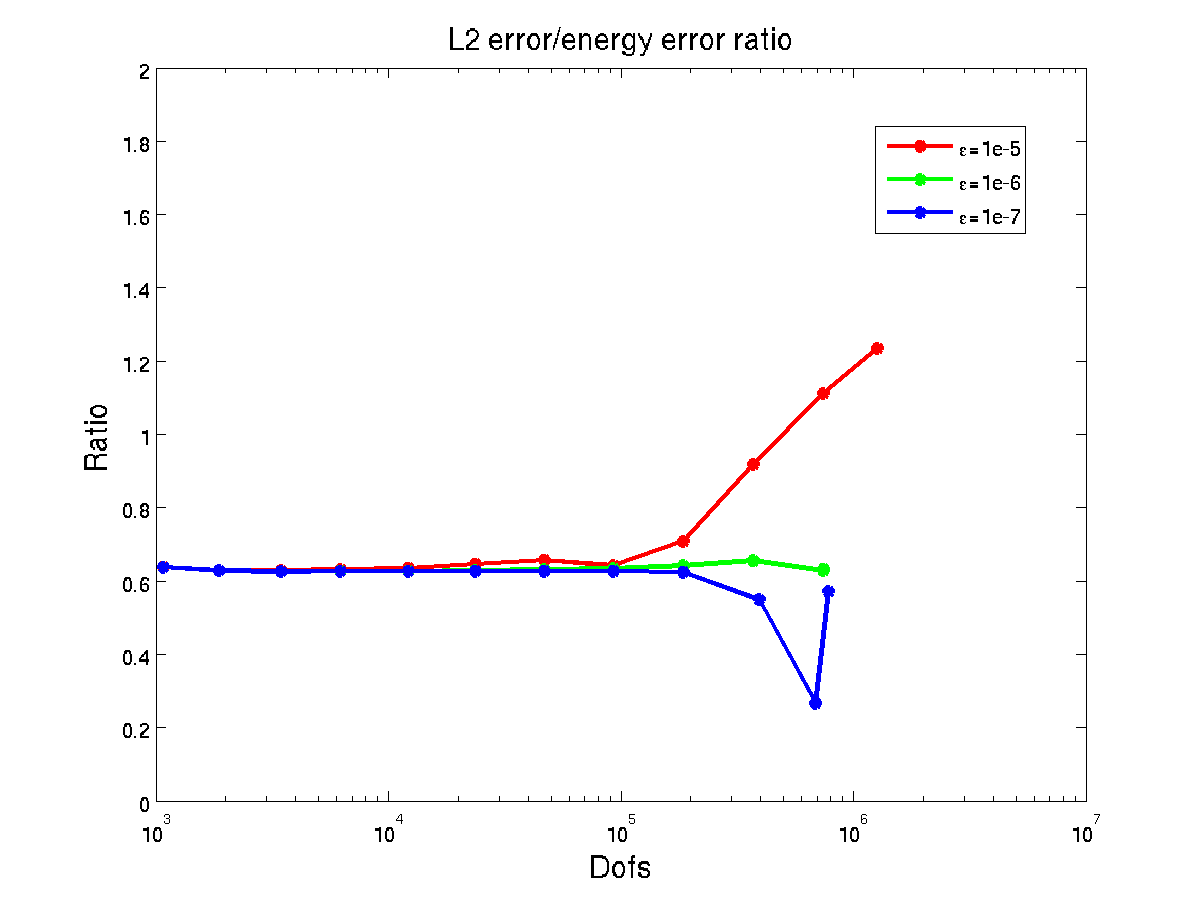
\includegraphics[scale=.36]{figs/roundoff_ratio.png}
}
\caption{Energy error and $L^2$/energy error ratio for $\epsilon=1e-5$, $\epsilon=1e-6$, $\epsilon=1e-7$. Non-monotonic behavior of the energy error indicates conditioning issues and roundoff effects.}
\label{roundoff_figures}
\end{figure}

Without anisotropic refinements, it still becomes computationally difficult to fully resolve the solution for $\epsilon$ smaller than $1e-5$. Regardless, for all ranges of $\epsilon$, DPG does not lose robustness, as indicated by the rates and ratio between $L^2$ and energy error in Figure~\ref{roundoff_figures} remaining bounded from both above and below. For $\epsilon = 1e-5$, we observe that the ratio of $L^2$ error increases, corresponding to the scaling of the test norm with mesh size (the transition in test norm occurs after 8 refinements, which, for an initial $4\times 4$ mesh, implies a minimum element size of about $1.5e-05$. At this point, rescaled test norm allows us to take advantage of the full magnitude of the $L^2$ term for $\|v\|$ and $\|\tau\|$ implied by our adjoint estimates). By analogy, for smaller $\epsilon = 1e-6, 1e-7$, the transition period should begin near the 10th and 11th refinement iterations; however, we do not observe such behavior, possibly due to roundoff effects. 
For $\epsilon=1e-6$, the ratio simply remains constant, but for $\epsilon=1e-7$, we observe definite roundoff effects, as the energy error increases at the 11th refinement. Since DPG is optimal in the energy norm for a mesh-independent test norm\footnote{While the test norm changes with the mesh, it increases monotonically. A strictly stronger test norm implies $\frac{b(u,v)}{\|v\|_1} \geq \frac{b(u,v)}{\|v\|_2}$ for any $\|v\|_1 \leq \|v\|_2$}, we expect monotonic decrease of the energy error with mesh refinement. Non-monotonic behavior indicates either approximation or roundoff error, and as we observed no qualitative difference between using $\Delta p = 5$ and $\Delta p = 6$ for these experiments, we expect that the approximation error is negligible and conclude roundoff effects are at play when these phenomena are observed. 

It is worth noting that for $\epsilon \leq 1e-5$, we do not perform enough refinements to completely resolve the boundary layer, so $|K| \geq \epsilon$ for all $K\in \Oh$. Thus, any roundoff effects observed are not due to the conditioning issues associated with the differing scales of the $\nor{v}_{L^2(K)}$ and $\nor{\grad v}_{L^2(K)}$ terms discussed previously. 

\subsection{Neglecting $\sigma_n$}

In practice, we will not have prior knowledge of $\sigma_n$ at the inflow, and will have to set $\beta_n u - \sigma_n = u_0$, ignoring the viscous contribution to the boundary condition.  The hope is that for small $\epsilon$, this omission will be negligible. Figure~\ref{ratios_noSigma} indicates that, between $\epsilon = .005$ and $\epsilon = .001$, the omission of $\sigma_n$ in the boundary condition becomes negligible, and both our error rates and ratios of $L^2$ to energy error become identical to the case where $\sigma_n$ is explicitly accounted for in the inflow condition. For large $\epsilon = .01$, the $L^2$ error stagnates around $1e-3$, or about $7\%$ relative error. 

\begin{figure}[h!]
\centering
\subfigure{
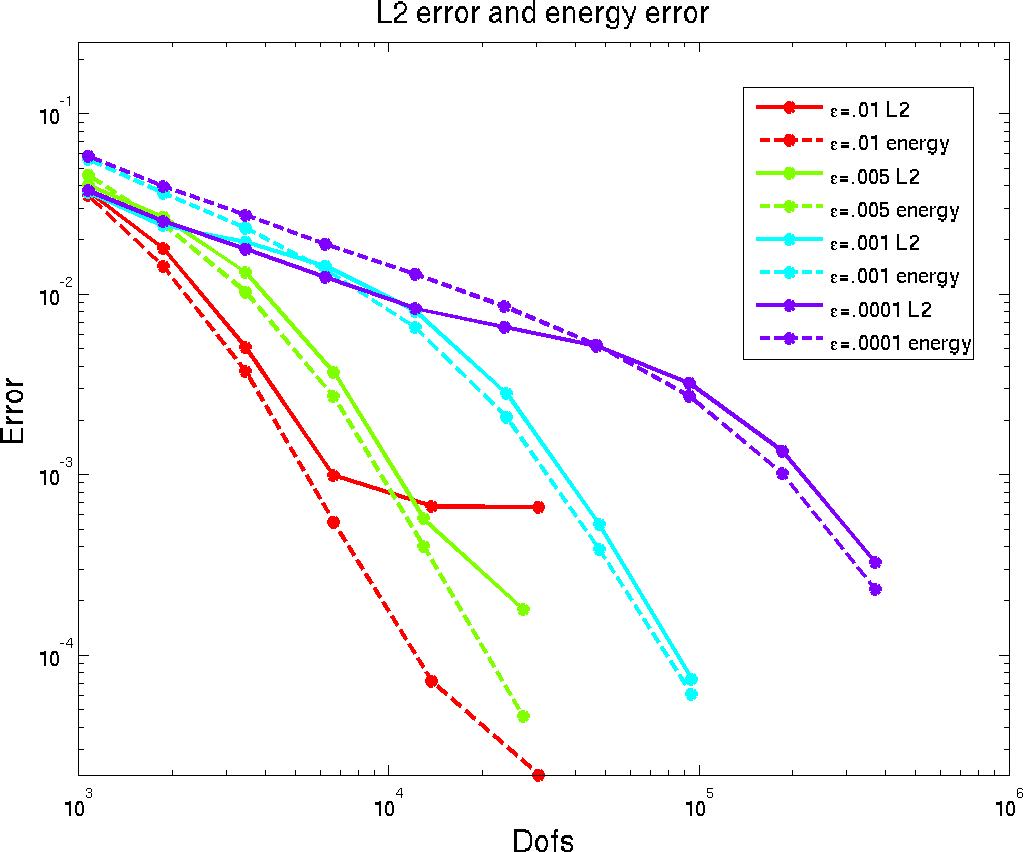
\includegraphics[scale=.38]{figs/rates_noSigma.png}
}
\subfigure{
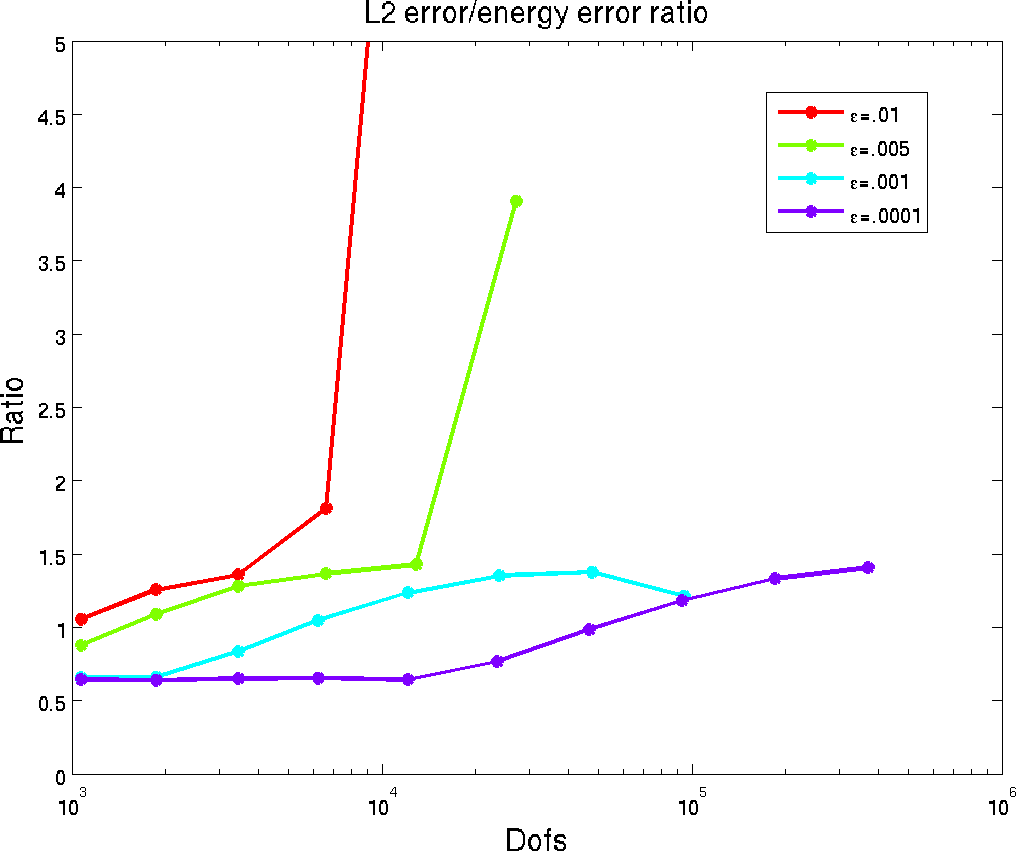
\includegraphics[scale=.38]{figs/ratio_noSigma.png}
}
\caption{$L^2$ and energy errors and their ratio when neglecting $\sigma_n$ at the inflow.}
\label{ratios_noSigma}
\end{figure}

\subsection{Discontinuous inflow data}

We note also that an additional advantage of selecting this new boundary condition is a relaxation of regularity requirements: as $\widehat{f}_n \in H^{-1/2}(\Gh)$, strictly discontinuous inflow boundary conditions are no longer ``variational crimes".  We consider the discontinuous inflow condition
\[
u_0(y) = \begin{cases}
(y-1)^2, \quad &y>.5\\
-y^2, \quad &y\leq .5 
\end{cases}
\]
as an example of a more difficult test case. 

\begin{figure}[h!]
\centering
\subfigure{
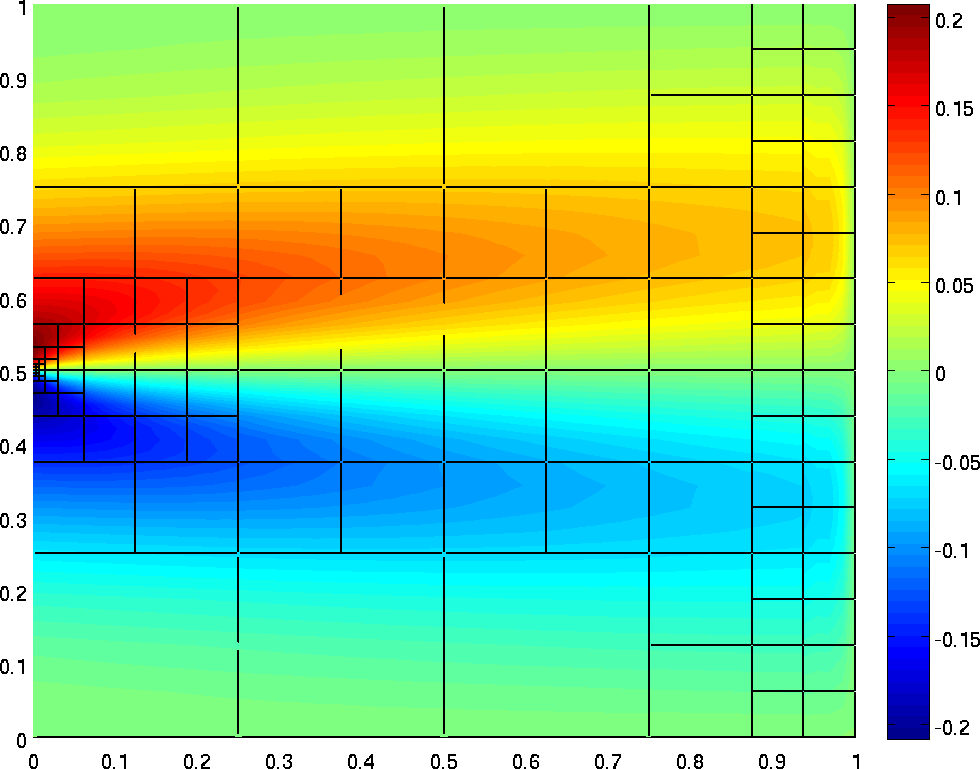
\includegraphics[scale=.38]{figs/disc_hat.png}
}
\subfigure{
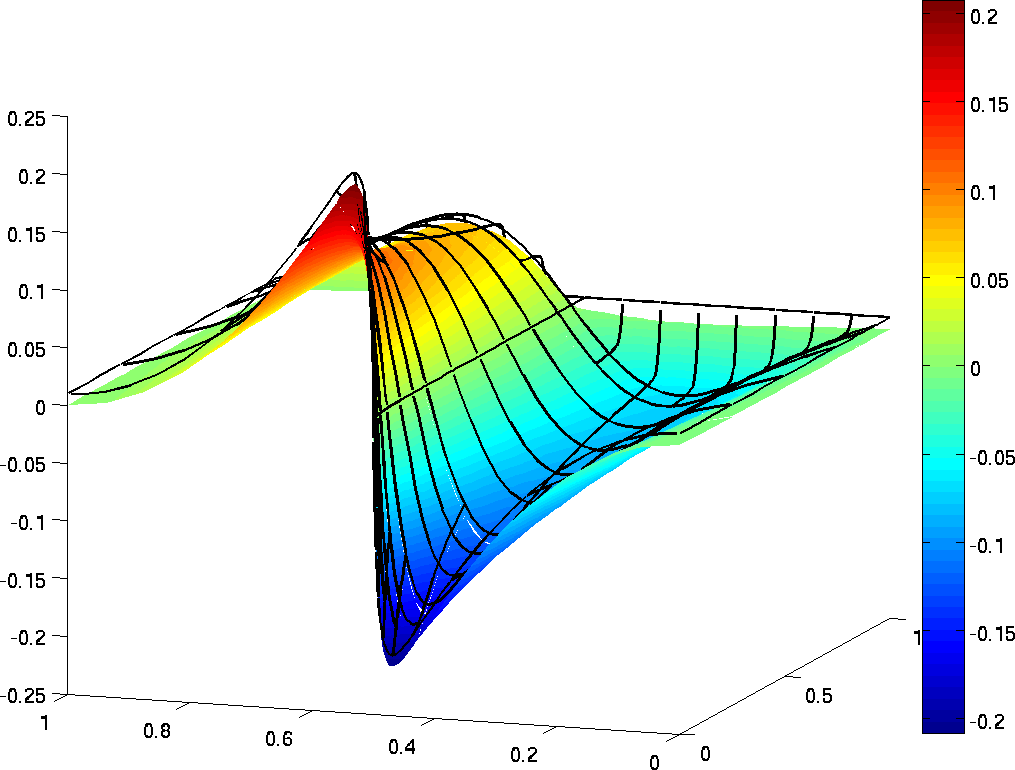
\includegraphics[scale=.38]{figs/disc_hat_surf.png}
}
\caption{Solution variables $u$ and $\widehat{u}$ with discontinuous inflow data $u_0$ for $\epsilon = .01$.}
\label{disc_sol}
\end{figure}
Figure~\ref{disc_sol} shows the solution $u$ and overlaid trace variable $\widehat{u}$, which both demonstrate the regularizing effect of viscosity on the discontinuous boundary condition at $x=0$. However, we do not have a closed-form solution with which to compare results for a stricly discontinuous $u_0$.  In order to analyze convergence, we approximate $u_0$ with 20 terms of a Fourier series, giving a near-discontinuity for $u_0$.  

\begin{figure}[h!]
\centering
\subfigure{
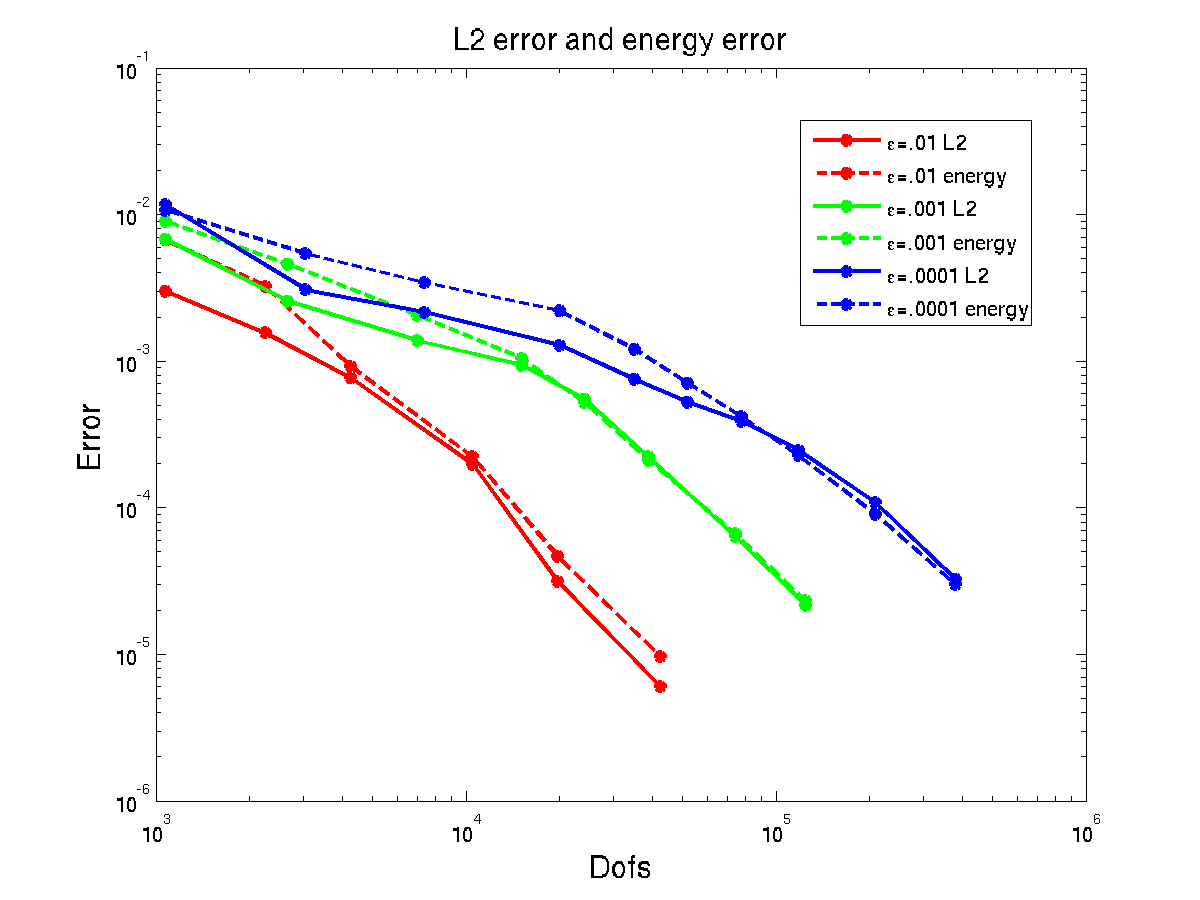
\includegraphics[scale=.36]{figs/rates_disc.png}
}
\subfigure{
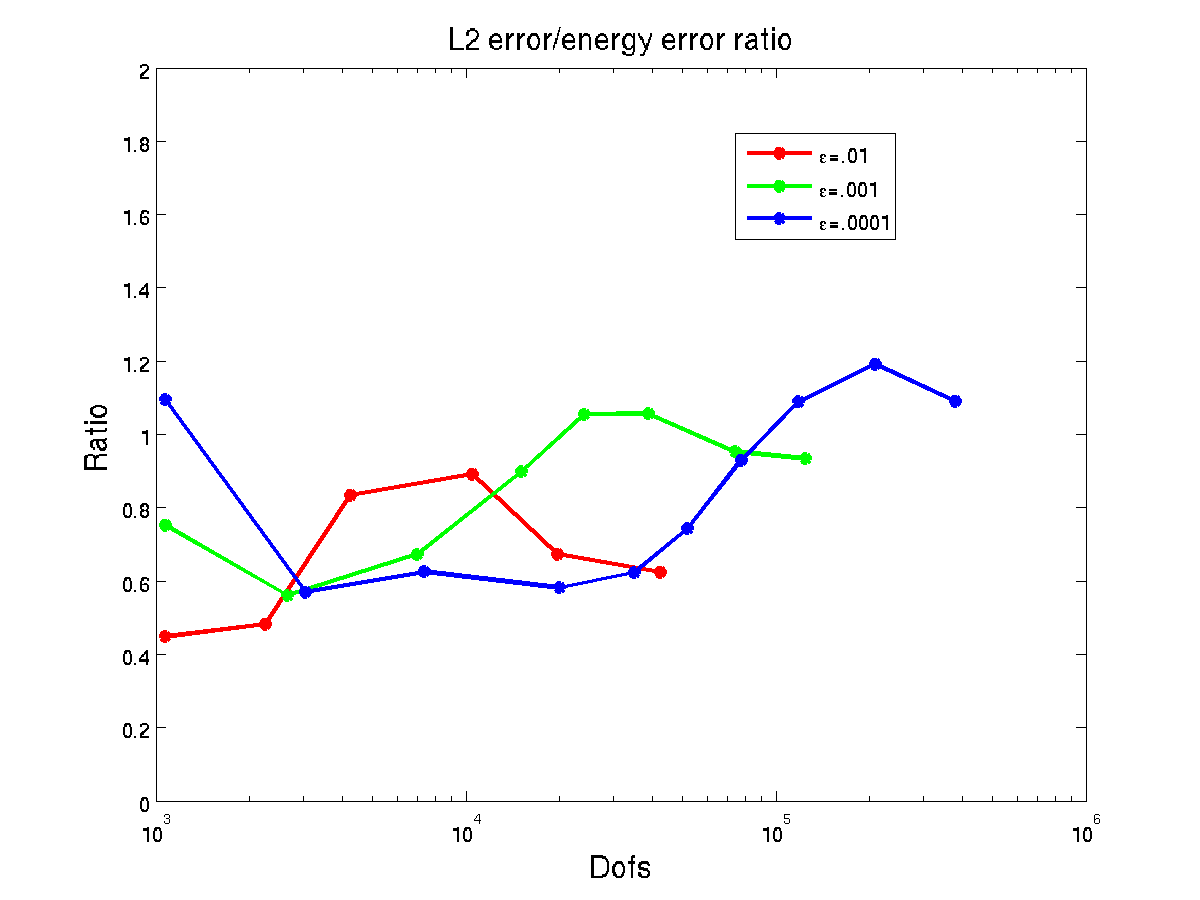
\includegraphics[scale=.36]{figs/ratio_disc.png}
}
\caption{$L^2$ and energy errors, and their ratio for $\epsilon=.01$, $\epsilon=.001$, $\epsilon=.0001$, with discontinuous $u_0$ approximated by a Fourier expansion. }
\label{disc_sol_fourier}
\end{figure}

The ratios of $L^2$ to energy error are now less predictable than for the previous example, in part due to the difficulty in approximating highly oscillatory boundary conditions. The numerical experiments were originally performed by applying boundary conditions via interpolation; the result was that the highly oscillatory inflow boundary condition was not sampled enough to be properly resolved, causing the solution to converge to a solution different than the exact solution.  The experiments were repeated using the penalty method to enforce inflow conditions; however, we note that the proper way to do so is to use an $L^2$ projection at the boundary.  Even when using the penalty method, however, the ratios still remain bounded and close to $1$ for $\epsilon$ varying over two orders of magnitude, as predicted by theory. 

